%% March 2018
%%%%%%%%%%%%%%%%%%%%%%%%%%%%%%%%%%%%%%%%%%%%%%%%%%%%%%%%%%%%%%%%%%%%%%%%%%%%
% AGUJournalTemplate.tex: this template file is for articles formatted with LaTeX
%
% This file includes commands and instructions
% given in the order necessary to produce a final output that will
% satisfy AGU requirements, including customized APA reference formatting.
%
% You may copy this file and give it your
% article name, and enter your text.
%
%
% Step 1: Set the \documentclass
%
% There are two options for article format:
% 
% PLEASE USE THE DRAFT OPTION TO SUBMIT YOUR PAPERS.
% The draft option produces double spaced output.
%

%% To submit your paper:
\PassOptionsToPackage{inline}{trackchanges}
\documentclass[draft]{agujournal2018}
\usepackage{apacite} 
\usepackage{comment}
\usepackage{url} %this package should fix any errors with URLs in refs.
\usepackage{lineno}
\linenumbers
%%%%%%%
% As of 2018 we recommend use of the TrackChanges package to mark revisions.
% The trackchanges package adds five new LaTeX commands:
%
%  \note[editor]{The note}
%  \annote[editor]{Text to annotate}{The note}
%  \add[editor]{Text to add}
%  \remove[editor]{Text to remove}
%  \change[editor]{Text to remove}{Text to add}
%
% complete documentation is here: http://trackchanges.sourceforge.net/
\addeditor{EC}
\addeditor{OF}

%%%%%%%

%% Enter journal name below.
%% Choose from this list of Journals:
%
% JGR: Atmospheres
% JGR: Biogeosciences
% JGR: Earth Surface
% JGR: Oceans
% JGR: Planets
% JGR: Solid Earth
% JGR: Space Physics
% Global Biogeochemical Cycles
% Geophysical Research Letters
% Paleoceanography and Paleoclimatology
% Radio Science
% Reviews of Geophysics
% Tectonics
% Space Weather
% Water Resources Research
% Geochemistry, Geophysics, Geosystems
% Journal of Advances in Modeling Earth Systems (JAMES)
% Earth's Future
% Earth and Space Science
% Geohealth
%
% ie, \journalname{Water Resources Research}
\journalname{JGR: Solid Earth}


\begin{document}

%% ------------------------------------------------------------------------ %%
%  Title
% 
% (A title should be specific, informative, and brief. Use
% abbreviations only if they are defined in the abstract. Titles that
% start with general keywords then specific terms are optimized in
% searches)
%
%% ------------------------------------------------------------------------ %%

% Example: \title{This is a test title}

\title{Effects of pre-existing structures on the seismicity of the Charlevoix Seismic Zone}

%% ------------------------------------------------------------------------ %%
%
%  AUTHORS AND AFFILIATIONS
%
%% ------------------------------------------------------------------------ %%

% Authors are individuals who have significantly contributed to the
% research and preparation of the article. Group authors are allowed, if
% each author in the group is separately identified in an appendix.)

% List authors by first name or initial followed by last name and
% separated by commas. Use \affil{} to number affiliations, and
% \thanks{} for author notes.  
% Additional author notes should be indicated with \thanks{} (for
% example, for current addresses). 

% Example: \authors{A. B. Author\affil{1}\thanks{Current address, Antarctica}, B. C. Author\affil{2,3}, and D. E.
% Author\affil{3,4}\thanks{Also funded by Monsanto.}}

\authors{Oluwaseun Idowu Fadugba\affil{1}, Eunseo Choi\affil{1}, and Christine A. Powell\affil{1}}

% \affiliation{1}{First Affiliation}
% \affiliation{2}{Second Affiliation}
% \affiliation{3}{Third Affiliation}
% \affiliation{4}{Fourth Affiliation}

\affiliation{1}{Center for Earthquake Research and Information, The University of Memphis, Memphis, TN 38152}
%(repeat as many times as is necessary)

%% Corresponding Author:
% Corresponding author mailing address and e-mail address:

% (include name and email addresses of the corresponding author.  More
% than one corresponding author is allowed in this LaTeX file and for
% publication; but only one corresponding author is allowed in our
% editorial system.)  

% Example: \correspondingauthor{First and Last Name}{email@address.edu}

\correspondingauthor{Oluwaseun Idowu Fadugba}{ifadugba@memphis.edu}

%% Keypoints, final entry on title page.

% Example: 
% \begin{keypoints}
% \item	List up to three key points (at least one is required)
% \item	Key Points summarize the main points and conclusions of the article
% \item	Each must be 100 characters or less with no special characters or punctuation 
% \end{keypoints}

%  List up to three key points (at least one is required)
%  Key Points summarize the main points and conclusions of the article
%  Each must be 100 characters or less with no special characters or punctuation 

\begin{keypoints}
  
  \item The CSZ seismicity and stress orientations are the combined effects of the rift faults and the impact \change[OF]{crater}{structure}.

  \item Planar faults we considered can explain the observed seismicity but only 50$\%$ of the stress rotation.

  \item \change[OF]{A crater}{An impact structure} four times less elastically stiff than the surrounding crust can explain the seismicity in the CSZ.
  
\end{keypoints}

%% ------------------------------------------------------------------------ %%
%
%  ABSTRACT
%
% A good abstract will begin with a short description of the problem
% being addressed, briefly describe the new data or analyses, then
% briefly states the main conclusion(s) and how they are supported and
% uncertainties. 
%% ------------------------------------------------------------------------ %%

%% \begin{abstract} starts the second page 

\begin{abstract}
The Charlevoix Seismic Zone (CSZ) \change[OF]{occurs}{is located} along the early Paleozoic St. Lawrence rift zone in southeastern Quebec at the location of a major Devonian impact \change[OF]{crater}{structure}. The \change[OF]{crater}{impact structure} superimposed major, steeply dipping basement faults trending \add[OF]{approximately} N35$^\circ$E. \change[OF]{Many}{Approximately 250} earthquakes are recorded each year \remove[OF]{in the CSZ} and are concentrated within and beneath the impact \change[OF]{crater}{structure}. \change[OF]{Some large-magnitude}{Most M4+} earthquakes associated with the rift faults occurred outside the \change[OF]{crater}{impact structure}. Apart from the unique distribution of earthquakes \remove[OF]{in the CSZ}, stress inversion of focal mechanisms shows stress rotations within the CSZ, and in the CSZ relative to the stress orientation determined from borehole breakouts. The primary goal of this research is to investigate the combined effects of the pre-existing structures and regional stresses on earthquake activity and stress rotations in the CSZ. We approach this using PyLith, a finite-element code for simulations of crustal deformation. Adopting the results from recent hypocenter relocation and 3D tomography studies, we modify the locations and dips of the rift faults and assess the effect of the new fault geometries on stress distributions. We also discuss the effects of resolved velocity anomalies. We find that the observed stress rotation is due to the combined effect of the rift faults and the \change[OF]{crater impact}{impact structure}. 1D velocity models of the CSZ with an embedded \change[OF]{crater}{impact structure} and a combination of 65$^\circ$-40$^\circ$-40$^\circ$ and constant 70$^\circ$ \change[OF]{fault dip}{fault-dip} models with a \add[OF]{very low} friction coefficient of 0.3 and cohesion of 0 MPa can explain the observed seismicity and more than 50$\%$ of the stress rotations.
\end{abstract}


\section{Introduction}
The Charlevoix Seismic Zone (CSZ) is the most seismically active region in eastern Canada. The CSZ is within the \change[OF]{Cambro-Ordovician}{Late Precambrian} St. Lawrence rift zone in southeastern Quebec and is overprinted by a Devonian impact \change[OF]{crater}{structure} (Fig. \ref{figone}). The impact \change[OF]{crater}{structure} has a radius of 28 km and is \change[OF]{15}{approximately 12} km deep~\citep{RONDOT1994}. The \change[OF]{crater}{impact structure} has a more damaged interior zone with a surface radius of 18 km (Fig. \ref{figone}). The impact \change[OF]{crater}{structure} is superimposed on three major rift faults trending N35$^\circ$E and dipping to the southeast~\citep{anglin1984,Rondot_1971}. The CSZ \change[OF]{is considered to pose a high risk of seismic hazard}{has high risk of seismic hazards} due to its history of generating \change[OF]{large}{moderate to large} earthquakes \citep{anglin1984,lamontagne1999}. Over 200 earthquakes are recorded each year in the CSZ (Nuttli magnitude, mN \add[OF]{mostly} $\leq$ 3) \citep{Baird_2010} and the hypocenters have a bimodal distribution with peaks at 10 and 22 km depths \citep{Vlahovic_2003}. The vast majority of earthquakes in the CSZ occur within the volume bounded by the rift faults \citep{Yu_2016} and those with greater magnitudes occur northeast of the \change[OF]{crater}{impact structure}~\citep{Mazzotti_2010} (Fig. \ref{figone}).

\begin{figure}[h]
\centering
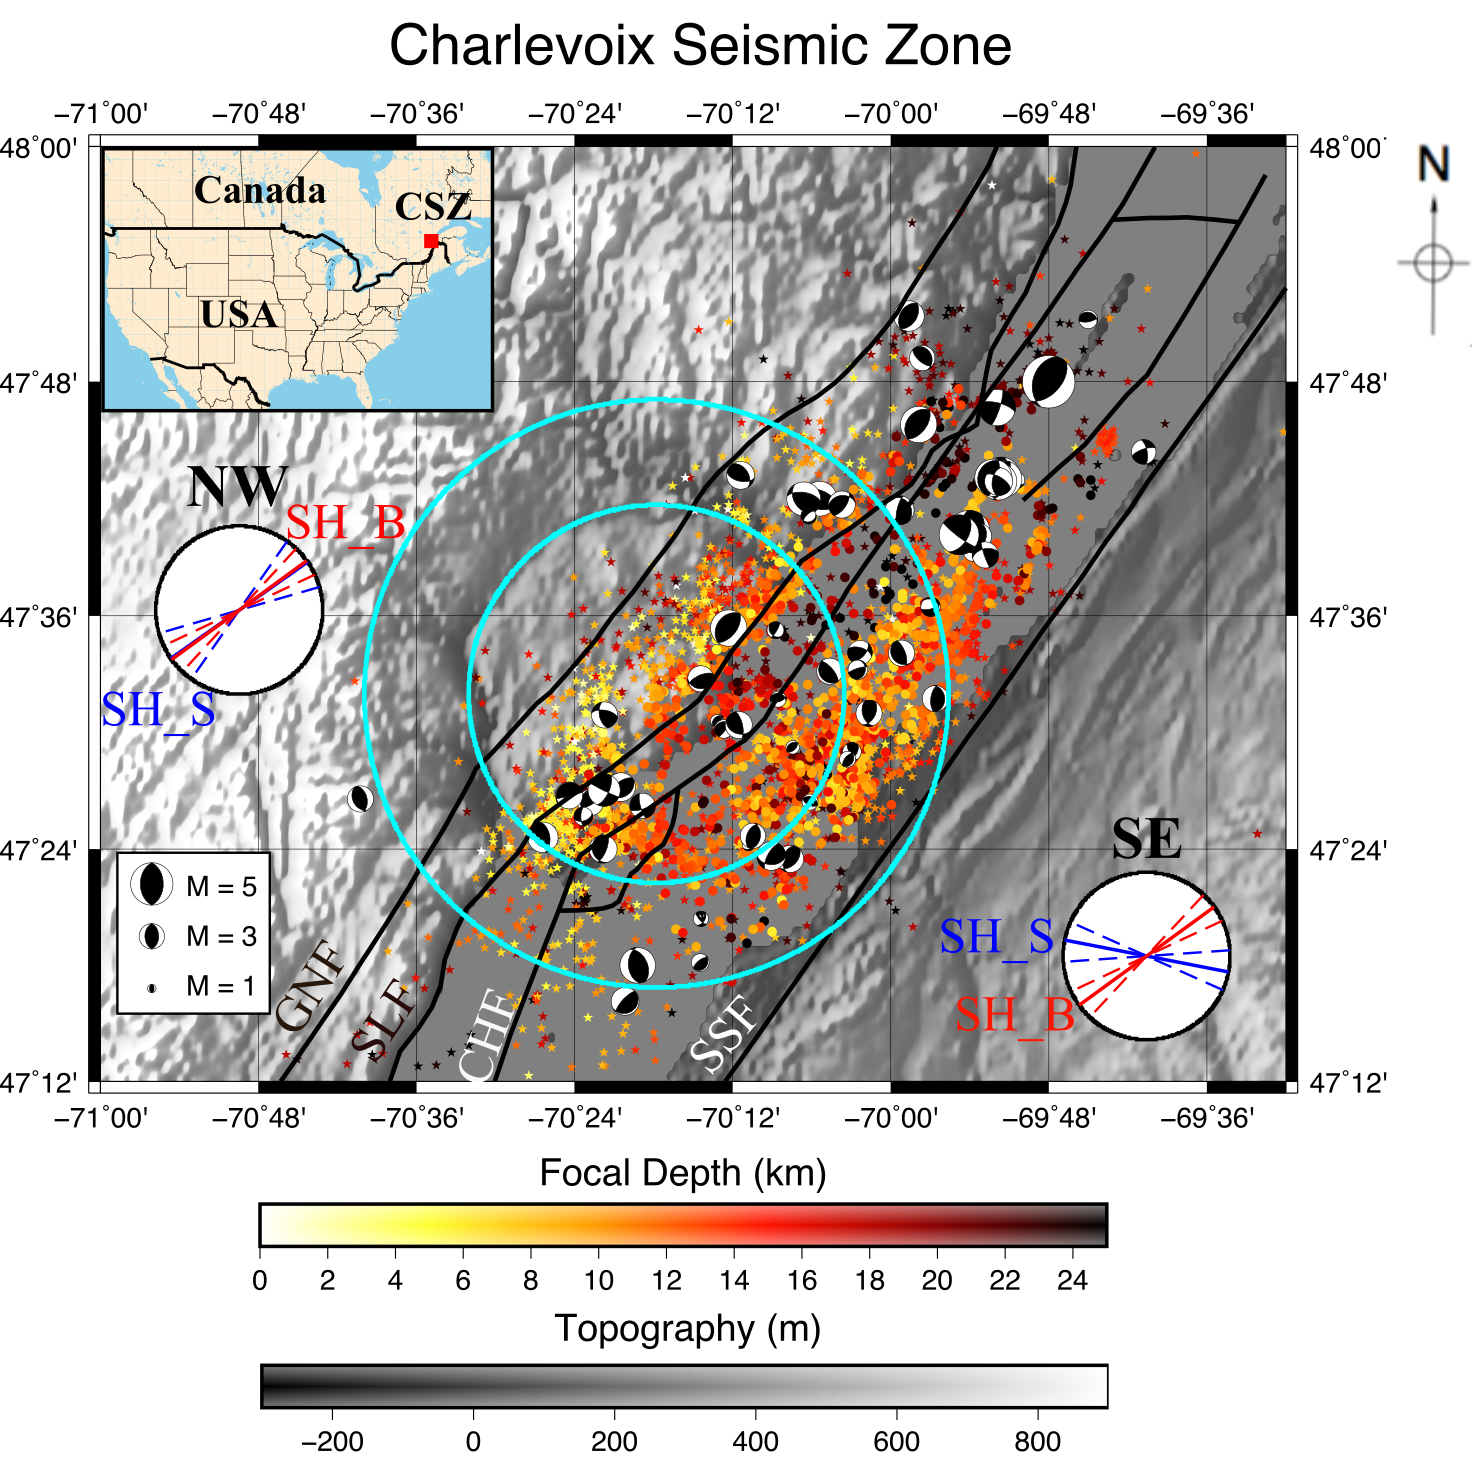
\includegraphics[width=18.5pc]{Map_of_CSZ_2.png} 
\caption{Topography\add[OF]{, bathymetry,} and seismicity of the Charlevoix Seismic Zone (CSZ) as well as the locations of the impact \change[OF]{crater}{structure} (outer cyan circle) and the more damaged inner \change[OF]{crater}{impact structure} (inner cyan circle). Small circles \add[OF]{and stars} are the relocated epicenters~\citep{Powell_2017} \add[OF]{and the complete dataset for the years 1988-2011, respectively,} and their colors represent the focal depths. The focal mechanisms are for the earthquakes used by \citet{Mazzotti_2010} for the stress inversion. Large circles labeled as NW and SE show orientations of SH$_{\max}$ from the stress inversion of focal mechanism (SH$_S$) and from borehole breakout measurements (SH$_B$) for the earthquake clusters northwest and southeast of the \change[OF]{crater}{impact structure} center. Solid black lines mark the rift faults known in the region: GNF, Gouffre Northwest Fault; SLF, Saint-Laurent fault; CHF, Charlevoix Fault; and SSF, South Shore Fault \citep{Rondot_1971,lamontagne1999}. The inset shows the location of the CSZ in eastern Canada. Earthquake \change[OF]{epicenters}{dataset} from the National Resources Canada catalog for the years 1988-2011.}
\label{figone}
\end{figure}

\citet{Vlahovic_2003} conducted a three-dimensional (3D) P-wave velocity study of the CSZ. The tomography model shows several \change[OF]{high-velocity}{higher P-wave velocity} bodies at mid-crustal depths. A significant fraction of the CSZ earthquakes occurs around these \change[OF]{high-velocity}{higher P-wave velocity} bodies and some larger earthquakes occur along the northern edges of the high velocity bodies. 

A recent earthquake relocation and tomography study of \citet{Powell_2017} using a larger number of CSZ earthquakes gives a better constraint on the geometries of these high-velocity bodies. In addition to the high-velocity bodies, \citet{Powell_2017} show that the relocated earthquakes are distributed along the rift faults and thus define the geometry of the rift faults. They also conclude that the dip of the northernmost rift fault is 65$^\circ$SE while the two other major faults dip 40$^\circ$SE. 

\citet{Mazzotti_2010} determined the orientation of maximum principal horizontal stress (SH$_{\max}$) from a stress inversion of focal mechanisms in ten seismic zones in central and eastern North America including the CSZ. They found a clockwise rotation of SH$_{\max}$ in the CSZ by about 32$^\circ$ relative to the regional SH$_{\max}$ orientation of 54$^\circ$ determined from borehole breakouts \citep{Zoback_1992,Mazzotti_2010}. \citet{Mazzotti_2010} observed a number of relative stress rotations in SH$_{\max}$ determined from different partitions of the earthquakes in the CSZ. The largest stress rotation occurs in the cluster of earthquakes located southeast of the \change[OF]{crater}{impact structure} midpoint relative to the earthquakes in the northwest of the \change[OF]{crater}{impact structure} midpoint. Specifically, SH$_{\max}$ in the cluster of earthquakes located southeast of the \change[OF]{crater}{impact structure} midpoint shows about a 47$^\circ$ clockwise rotation whereas the cluster located to the northwest has a SH$_{\max}$ that is compatible with the regional SH$_{\max}$~\citep{Mazzotti_2010} (Fig. \ref{figone}).

\citet{Baird_2010} explain the distribution of seismicity in the CSZ as products of the interactions between the impact structure and the rift faults. Their numerical models for the rift faults and impact \change[OF]{crater}{structure} subjected to the regional stress show increased differential stresses near the fault planes, which is consistent with the distribution of the earthquakes. Stress solutions from their numerical models show greater differential stress in the northeast of the \change[OF]{crater}{impact structure}, where \change[OF]{more}{most of the larger} earthquakes occur, than in the southwest. However, their models could not fully explain the SH$_{\max}$ rotations in the CSZ relative to the regional SH$_{\max}$. Instead, they addressed the observed stress rotations based on the discrepancy between the SH$_{\max}$ from the stress solutions in the seismogenic zone and the SH$_{\max}$ inverted from the modeled slips on the rift faults.

In this study, we present a new set of numerical models that can assess the impacts \change[OF]{on}{of} stress distribution due to fault geometry, frictional strengths of faults, elastic properties of the \change[OF]{crater}{impact structure} and velocity models for the region. We then try to correlate modeled stress distributions with the recently-relocated hypocenters \citep{Powell_2017} and discuss implications for the non-uniform stress orientation around the \change[OF]{crater}{impact structure} that was previously recognized.

%%%%%%%%%%%%%%%%%%%%%%%%%%%%%%%%%%%%%%%%%%%%%%%
\section{Model Setup}
We create numerical models that include three major rift faults and the damaged impact \change[OF]{crater}{structure} (Fig. \ref{figtwo}A). For this purpose, we use PyLith version 2.1.0~\citep{Aagard2015, matthew2015, c2015}, an open-source finite element code for modeling dynamic and quasi-static tectonic deformation. PyLith is suitable for the intended models because it can compute elastic responses of a model involving multiple faults and material heterogeneities subjected to various types of loading.

\subsection{Model geometry}
Our models are composed of three units, crust, \change[OF]{crater}{impact structure} and rift faults, reflecting a simplification of the geology of the region (Fig. \ref{figtwo}A). The crust is a 220 $\times$ 220 $\times$ 40 km box with the \change[OF]{crater}{impact structure} cut out. The impact \change[OF]{crater}{structure} is modeled as a spherical cap with a surface diameter of 60 km and a depth of 15 km. 

The three rift faults have a strike of N35$^\circ$E and are embedded in the crust layer except for the top surface edge that is exposed on the surface. The three faults correspond to the Gouffre \add[OF]{NW} River, St. Laurent, and the Charlevoix faults (Fig. \ref{figone}). \citet{Baird_2010} modeled the Gouffre River, St. Laurent, and the South Shore faults. They did not model the Charlevoix fault. The locations of the rift faults relative to the \change[OF]{crater}{impact structure} are based on geologic maps by \citet{lamontagne1999} and \citet{Rondot_1971}. We create two sets of models with different dip angles of the faults based on two proposed geometries of the rift faults. One set has a uniform dip of 70$^\circ$SE for all three faults \citep{anglin1984,Baird_2010} while the other has 65$^\circ$, 40$^\circ$ and 40$^\circ$ for the three planar faults, from north to south, respectively \citep{Powell_2017}. 

We conducted resolution tests in which the change in displacement and stress solutions relative to a 1 km-resolution model are monitored as a function of element size. \change[OF]{Displacement was almost constant for 2 km or smaller element sizes}{Displacements and differential stresses do not change appreciably for elements sizes equal to 4 km or smaller (Fig. S1)}. \add[OF]{Based on the resolution tests, we use the element size of 2 km for most of the models and 4 km for more computationally expensive models like those for exploring the effects of the friction coefficient. Low-friction models, especially those with $\mu$ equal to 0.1 and 0.2, are very expensive due to slow convergence rate in the non-linear solution scheme. Running all the models in this group at the same mesh resolution of 4 km ensures intra-group consistency; and the comparison with 2 km-resolution models is also justified because the descritization error does not significantly increase as the resolution increases to 4 km (Fig. S1).} We also observe edge effects by comparing a 420 $\times$ 420 $\times$ 40 km model with the original 220 $\times$ 220 $\times$ 40 km model, finding that the seismogenic parts around the \change[OF]{crater}{impact structure} show consistent displacement and stress solutions for both domain sizes. Based on this result, we choose the smaller domain for this study and set the element size to be about 2 km. \add[OF]{The average computation time was about 16 days for fault models ($\mu$ = 0.3) with 2 km element size on 16 cores on the University of Memphis High Performance Computing cluster. The model with fault dips of 65$^\circ$-40$^\circ$-40$^\circ$ took about two times as long to run for the same model time. We do not clearly understand why the model with shallower-dipping faults is slower than the others roughly by a factor of two and further analyzing computational efficiency is beyond the scope of this paper.}
%we use an element size of 4 km for models with friction coefficient ($\mu$) values of 0.1 and 0.2 due to their expensive computation time.



\subsection{Initial and boundary conditions}
\label{Initial_and_boundary_conditions}
Initial stresses are assumed to be lithostatic but due to the non-planar geometry of the \change[OF]{crater}{impact structure}, computing initial lithostatic equilibrium stresses is not trivial. We first compute lithostatic stresses based on the density distribution from an adopted velocity model for the CSZ (Table~\ref{tableone}) and use it as an initial stress distribution. We then use this stress solution as the true initial stress conditions. We verify that this two-step approach leads to an initial stress field perfectly balancing the gravitational body force by observing that the initial vertical displacements are uniformly zero.

Velocities are prescribed on the sides perpendicular to the $x$-axis (Fig. \ref{figtwo}A) while the $y$-perpendicular sides and the bottom boundary are free-slip and the top boundary is traction-free. Rather than applying velocities oblique to the sides, we rotate the model domain such that the $x$-axis is oriented to N55$^\circ$E, the regional SH$_{\max}$ direction~\citep{Zoback_1992} (Fig. \ref{figtwo}B). We apply a 1 m/yr compressive velocity in the x-axis direction. The magnitude of boundary velocity does not represent any tectonic loading in the continental interiors but has the sole purpose of increasing the differential stress ($\sigma_D$ = $\sigma_1 - \sigma_3$). Noting that \change[OF]{most earthquakes in the crater occur near 10 km depth}{the depth distribution of earthquakes within the impact structure has a peak at 10 km} \citep{Baird_2010,Powell_2017}, we increase the boundary displacement until $\sigma_D$ reaches 706 MPa at 10 km depth based on Byerlee's law for dry rocks, $\tau$  = 50 MPa + 0.6$\,\sigma_n$~\citep{Byerlee_1978}. \add[OF]{More details of the full derivation of the stopping criterion for boundary loading is given in the supplementary information. We assume that} $\sigma_3$ corresponds to the lithostatic stress \change[OF]{. C}{and adopt the sign convention that compressive stress is negative.}

\begin{figure}[ht]
\centering
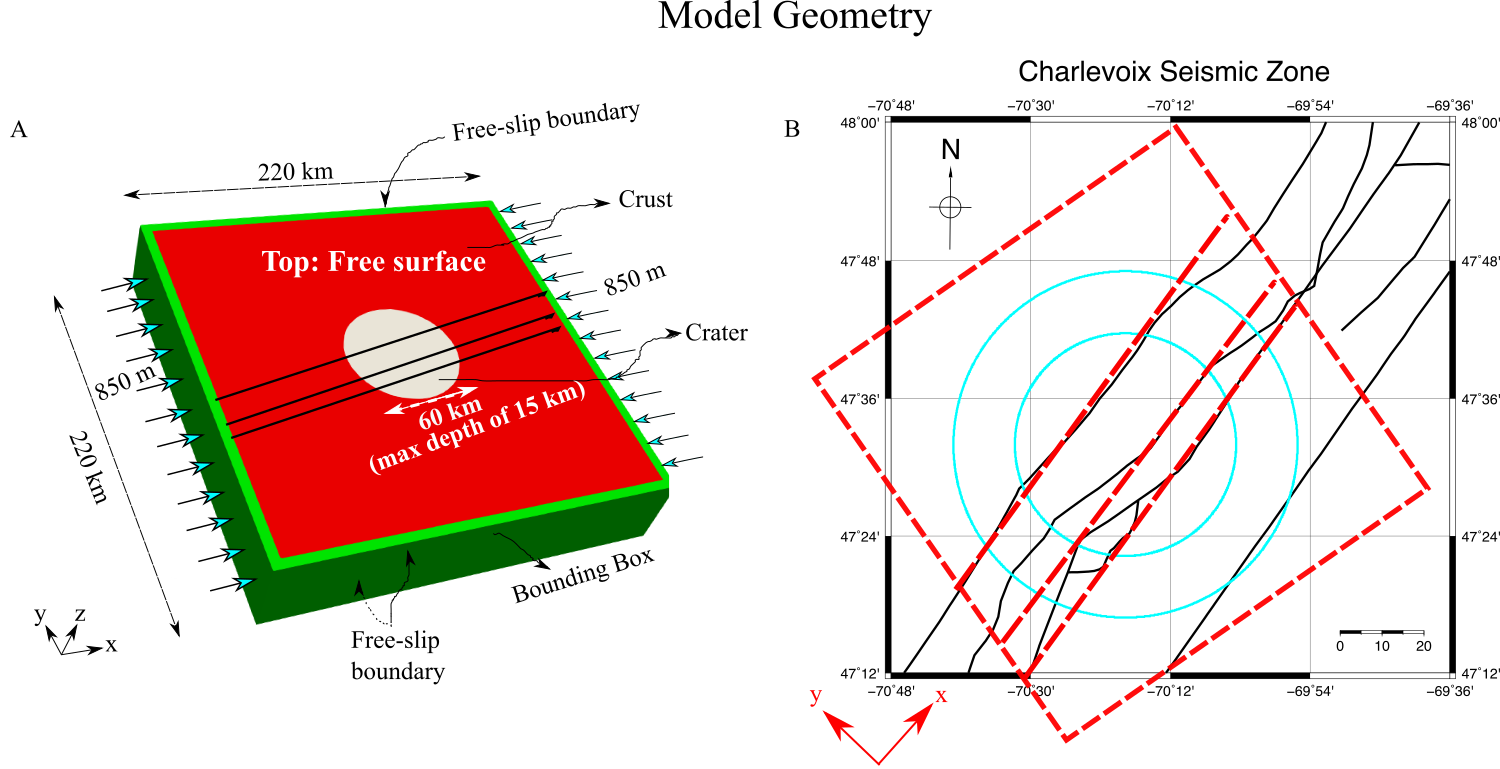
\includegraphics[width=25pc]{model_geometry.png}
\caption{(A) Model domain with the \change[OF]{crater}{impact structure} (gray) and crust (red). The three rift faults (black lines), dimensions, boundary conditions and the total amount of displacement are annotated. The outer 10 km-thick layer of crust (green) is added to contain fault edges within the domain, a requirement by PyLith. (B) The orientation of the model domain (red dotted box) and the associated coordinate axes (red arrows) relative to the geographic reference frame. The red dotted box is not the actual model domain but just a box that shows its "orientation." Cyan circles on the geographic map show the inner and outer \change[OF]{crater}{impact structure} boundaries and black solid lines trace rift faults (see Fig. \ref{figone}).}
\label{figtwo}
\end{figure}

\subsection{Elastic moduli from velocity models}
We assume linear elasticity for both crust and \change[OF]{crater}{impact structure}. To obtain elastic moduli and density distributions, we consider three regional velocity models and one recent model based on local earthquake tomography~\citep{Powell_2017}. The regional models are for the Saguenay region in Quebec~\citep{Somerville1990}, the 1D standardized halfspace velocity model of eastern Canada~\citep{lamontagne1999}, and the 1D velocity model derived from \change[OF]{seismic refraction studies}{a simultaneous inversion of hypocenters and velocities of the CSZ}~\citep{lamontagne1999} (Fig. \ref{figthree}).

\begin{figure}[ht]
\centering
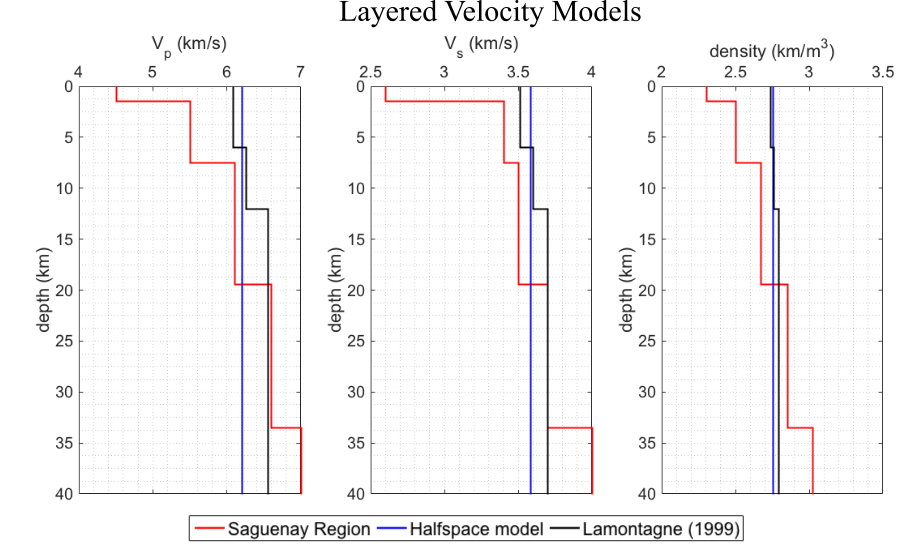
\includegraphics[width=30pc]{layered_vel_models.png}
\caption{Velocity models used in this study. Red, blue and black lines are velocity models for the Saguenay region \citep{Somerville1990}, \change[OF]{a standardized velocity}{the Geological Survey of Canada (GSC) standard velocity model} of Eastern Canada \citep{lamontagne1999} and the \add[OF]{Canadian Shield (North Shore)} velocity model of CSZ \citep{lamontagne1999}.}
\label{figthree}
\end{figure}

We also consider a non-uniform distribution of density and elastic moduli inferred from the 3D $V_p$ and $V_s$ tomography model by \citet{Powell_2017}, of which $V_p$ and $V_s$ variations for the depth range from 12 to 14 km are shown in Fig. \ref{figfour}. The tomography has a block size of 2 km and velocity features with a dimension of 6 km can be resolved. Since this tomography solution does not cover the entire study area, we assume a halfspace velocity model~\citep{lamontagne1999} outside of the tomography coverage. Smooth transition between the tomography model and the half-space model is achieved by linear interpolation. Densities ($\rho$) are computed according to Gardner's principle~\citep{Gardner_1974}: $\rho=0.31 V_p^{0.25}$, where $V_p$ is the P-wave velocity in m/s and density is given as g/cm$^3$.

For simplicity, we assume that the \change[OF]{crater}{impact structure}'s bulk and shear moduli are a certain fraction of those of the crust~\citep[e.g.,][]{Baird_2010}. Similarly, the density of the \change[OF]{crater}{impact structure} is reduced \remove[OF]{by 10 \%} from that of the 1D velocity models over the corresponding depth range \add[OF]{to model damaged crustal rocks. Models with density reduced by 0 to 20 \% were run but did not exhibit significant changes as shown in Fig. S3 in the supplementary information. All the models presented in this study have 10 \% of density reduction in the impact structure.}

\begin{figure}[ht]
\centering
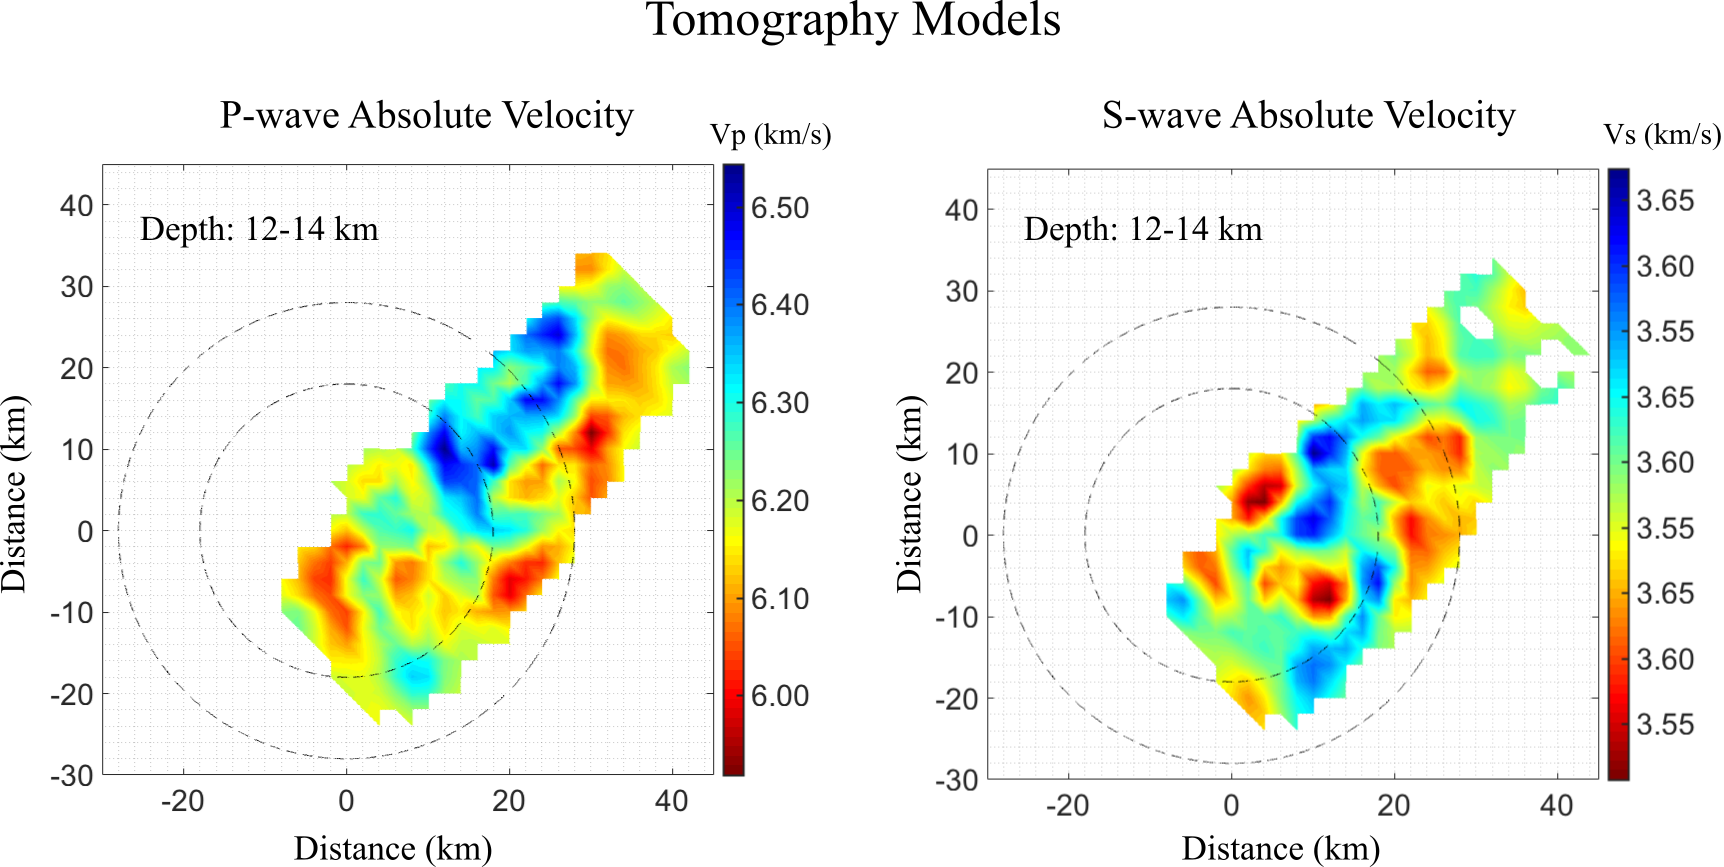
\includegraphics[width=30pc]{TOMO_vel_models.png}
\caption{Variation of $V_p$ and $V_s$ at the depths from 12 to 14 km from the 3D seismic tomographic model by \citet{Powell_2017}.}
\label{figfour}
\end{figure}

\subsection{Treatment of rift faults}
We treat the rift faults as cohesive-frictional planes, on which slip vectors are not prescribed but determined by the model. In order to create relative motions across the rift fault planes, PyLith decouples the motion of the two sides of the faults by inserting cohesive cells on the fault surfaces. We assign a coefficient of static friction ($\mu$) and the cohesion ($C$) on the fault. We assume that $\mu$ and $C$ are uniform on the fault planes in each model but investigate the consequences of varying $\mu$ from 0.1 to 0.6 at a constant $C$ of 0 MPa.  \add[OF]{Although cohesion values from 0 to 30 MPa have been tested and found to have significant effects, we choose to present models with zero cohesion in this study because it is appropriate for pre-existing faults with low normal stress}~\citep[e.g.,][]{Marone_Chris}. \add[OF]{We note that the deep portions of the model faults might not satisfy the condition of low normal stress and thus a further investigation on the depth-variation of cohesion is desirable.}
%\add[OF]{and slips on the model faults occur only down to about 10 km depth satisfying this condition.} 
%\note[EC]{I think the following sentences should be in discussion, not here.}\add[OF]{We ran a series of models in which the rift faults dip at 70$^{\circ}$ and the friction coefficient ($\mu$) is fixed to be 0.3 while cohesion ($C$) is one of 0, 3, 5, 10, 20 and 30 MPa (Fig. S4). Cohesion values less than 5 MPa could explain the spatial distribution of observed seismicity in the CSZ.} 

The reference model (SNFR25) has the geometry described above but without the rift faults. This is equivalent to a model with infinitely strong faults. The initial stress state is close to the initially assumed lithostatic stress after the nonplanar correction due to the \change[OF]{crater}{impact structure}. We determine the percentage change in differential stress, $\Delta\sigma_{D}^{\prime}=100\,( \sigma_{D}-\sigma_{D,ref}) / \sigma_{D,ref}$, and the change in the orientation of SH$_{max}$,  $\Delta\phi_{\max}=\phi_{\max}-\phi_{\max,ref}$, where $\phi_{\max}$ denotes the orientation of the maximum principal stress ($\sigma_1$). Since our model domain was rotated clockwise about the center of the \change[OF]{crater}{impact structure} by 35$^\circ$, $\phi_{\max}$ equal to zero should be understood as parallel to the regional stress field. Positive and negative values of $\phi_{\max}$ correspond to anticlockwise and clockwise rotation from the direction of applied loading, respectively. \add[OF]{In order to quantify the spatial correlation between the simulated stress changes and the earthquake hypocenters, we determine the percentage of hypocenters that fall within the region of $\Delta\sigma_{D}^{\prime} \ge$ 0.5 \%. We did not account for the uncertainty in hypocenter relocation and the effect of any along-strike variation in the fault dips.} % in reality


\subsection{Control Parameters}
We create a series of models in which the following parameters are varied: dips of the rift faults, friction coefficients, \change[OF]{crater}{impact structure}-crust elastic moduli ratios, and the velocity models. Two fault geometries for the CSZ are considered. One model has a dip angle of 70$^\circ$SE for all three rift faults \citep{Baird_2010}. The other assumes that the three faults have dip angles of 65$^\circ$SE, 40$^\circ$SE and 40$^\circ$SE from north to south~\citep{Powell_2017}.

\change[OF]{crater}{Impact structure}-crust elastic moduli ratios tested are 0.25, 0.5 and 1.0. When the modulus ratio is 1.0, the \change[OF]{crater}{impact structure} has the same velocity model as the crust. The friction coefficient, $\mu$, is varied from 0.1 to 0.6 at a constant cohesion of 0 MPa in one set of models. We assume that $\mu$ and $C$ are the same for the three rift faults and it is uniform on the fault planes, including the part of the faults within the \change[OF]{crater}{impact structure} region. 

Three velocity models are considered in this study: The 1D Saguenay velocity model~\citep{Somerville1990}, the 1D CSZ velocity model~\citep{lamontagne1999} and the 3D V$_p$ and V$_s$ tomography model~\citep{Powell_2017} (Figs. \ref{figthree} and \ref{figfour}). When the tomography model is used, the \change[OF]{crater}{impact structure}-crust moduli ratio becomes irrelevant. All the models presented in this paper are listed in Table~\ref{tableone}.


\begin{table}
\caption{List of numerical models} 
%\note[EC]{Each symbol needs a description. Cohesion needs a unit. I gave a try with the $\dagger$ symbol.}}
\centering
\begin{tabular}{llcccccc}
\hline
Model & Velocity Model & Dip of Rift Faults & Moduli ratio & $\mu^{\dagger}$ & $C^{\dagger}$ (MPa) & K$^{\dagger,*}$ (MPa) & G$^{\dagger,*}$ (MPa) \\
\hline
SNFR25  & Saguenay Region$^{1}$ & No faults & 0.25 & 0.3 & 0 & 55.7 & 32.7  \\
SD70R25  &  & $70^\circ-70^\circ-70^\circ$  & 0.25 & 0.3 & 0 & 55.7 & 32.7 \\
SD70R25V  &  & $70^\circ-70^\circ-70^\circ$  & 0.25 & 0.1-0.6 & 0 & 55.7 & 32.7 \\
%SD70R25M1 &  & $70^\circ-70^\circ-70^\circ$  & 0.25 & 0.1 & 0 \\
SD65R25  &  & $65^\circ-40^\circ-40^\circ$  & 0.25 & 0.3 & 0 & 55.7 & 32.7\\
SD70R50  &  & $70^\circ-70^\circ-70^\circ$  & 0.5 & 0.3 & 0 & 55.7 & 32.7 \\
SD70R100   &  & $70^\circ-70^\circ-70^\circ$  & 1.0 & 0.3 & 0 & 55.7 & 32.7 \\
LD70R25 & 1-D Model$^{2}$ & $70^\circ-70^\circ-70^\circ$ & 0.25 & 0.3  & 0 & 60.0 & 35.7 \\
TD70 & Tomography$^{3}$ & $70^\circ-70^\circ-70^\circ$ & - & 0.3 & 0 & 58.7 & 35.3 \\
\hline
\multicolumn{8}{l}{$^{1}$\citet{Somerville1990}. $^{2}$\citet{lamontagne1999}. $^{3}$\citet{Powell_2017}. $^{*}$K, G at 10 km depth.} \\
\multicolumn{8}{l}{$^{\dagger}$$\mu$, $C$, $K$ and $G$ are friction coefficient, cohesion, bulk and shear modulus, respectively.}

\end{tabular}
\label{tableone}
\end{table}


% ###################################################################################################################

\section{Results}

\subsection{Reference Model (SNFR25)} \label{Ref_Model}
The effects of the weaker \change[OF]{crater}{impact structure} are dominant in SNFR25. $\sigma_D$ is smaller by 100s MPa in the \change[OF]{crater}{impact structure} region relative to the surrounding crustal rock as shown by 5 and 10-km depth sections (Fig. \ref{fig:SNFR25_ref}A). The absolute value of $\sigma_D$ is greater (i.e. is more negative) in the direction perpendicular to the applied loading than in the parallel direction. At depths below the \change[OF]{crater}{impact structure} (i.e., depths $\ge$ 15 km), $\sigma_D$ is more negative at the central region by about 300 MPa relative to the average $\sigma_D$ at those depths (Fig. \ref{fig:SNFR25_ref}A). The higher negative value of $\sigma_D$ at 15 km depth decreases to the average value at that depth within 20 km from the center of the model geometry. The effect of the \change[OF]{crater}{impact structure} weakens at 20 km and eventually becomes insignificant at 25 km (Fig. \ref{fig:SNFR25_ref}A).

$\phi_{\max}$, the orientation of SH$_{\max}$, shows a four-lobe pattern of alternating polarities around the \change[OF]{crater}{impact structure} (Fig. \ref{fig:SNFR25_ref}B). $\phi_{\max}$ uniformly approaches 0$^\circ$, the loading direction, away from the \change[OF]{crater}{impact structure} and also with depth (Fig. \ref{fig:SNFR25_ref}B). In the SE corner of the \change[OF]{crater}{impact structure}, $\phi_{\max}$ shows a maximum clockwise (i.e., negative) rotation of about 18.3$^\circ$ from the regional stress direction (5 km panel in Fig. \ref{fig:SNFR25_ref}B). 
$\phi_{\max}$ at 5 km and 10 km depths is close to 0$^\circ$ within the \change[OF]{crater}{impact structure}, being subparallel to the regional stress orientation ~\citep{Zoback_1992}.

\begin{figure}[ht]
\centering
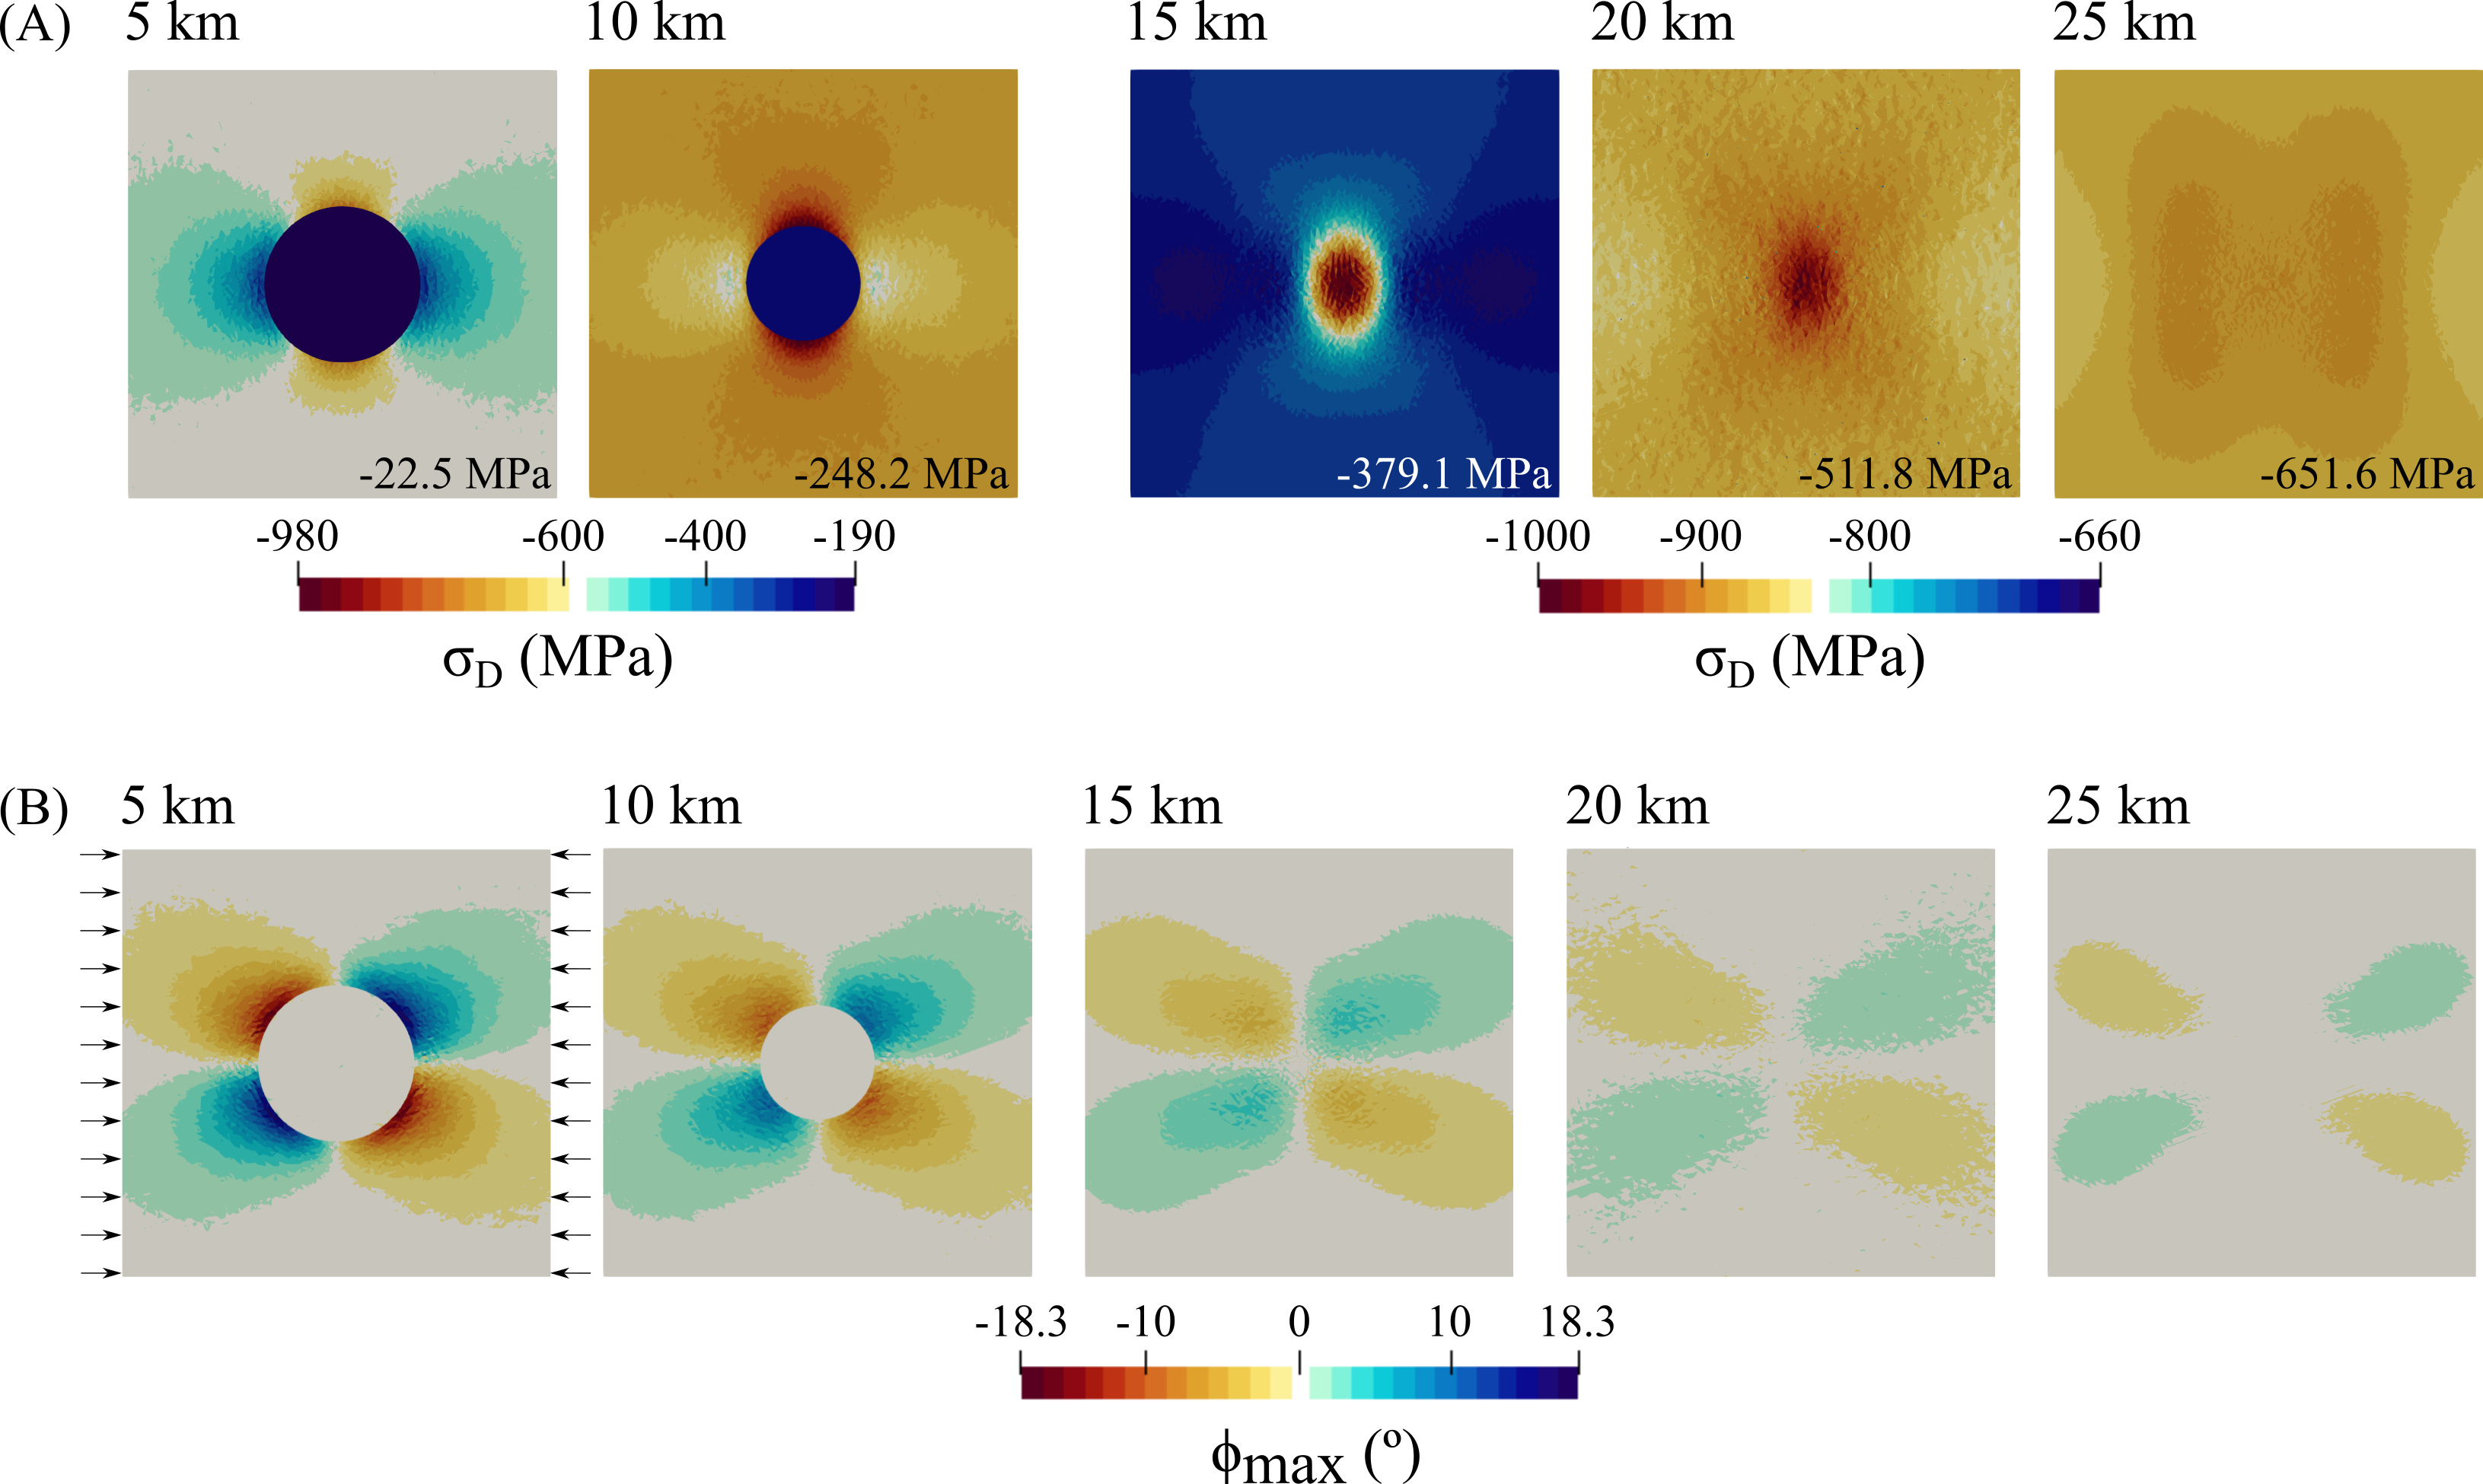
\includegraphics[width=30pc]{SNFR25.png}
\caption{(A) Differential stress ($\sigma_D$) and (B) SH$_{\max}$ orientation ($\phi_{\max}$) in the reference model (SNFR25) at different depths. The value of lithostatic stress at each depth is at the lower right corner of each depth slice in \ref{fig:SNFR25_ref}A. The arrows in \ref{fig:SNFR25_ref}B represent the loading direction for all models. Note the change in scale in \ref{fig:SNFR25_ref}A for depths greater than 10 km. Each figure is 70 $\times$ 70 km.} 
\label{fig:SNFR25_ref}
\end{figure} 

% #############################################################
\subsection{Effects of rift faults and their dip}
\subsubsection{SD70R25}
Magnitudes of $\sigma_{D}$ in SD70R25 are smaller in the \change[OF]{crater}{impact structure} than in the surrounding crust, as in the reference model, but also significantly modified by abrupt changes in the vicinity of the rift faults (Fig. \ref{fig:SD70R25}A). $\sigma_{D}$ at a distance greater than 50 km from the center of the \change[OF]{crater}{impact structure} is similar to that of the reference model at each depth. 

\begin{figure}[ht]
\centering
%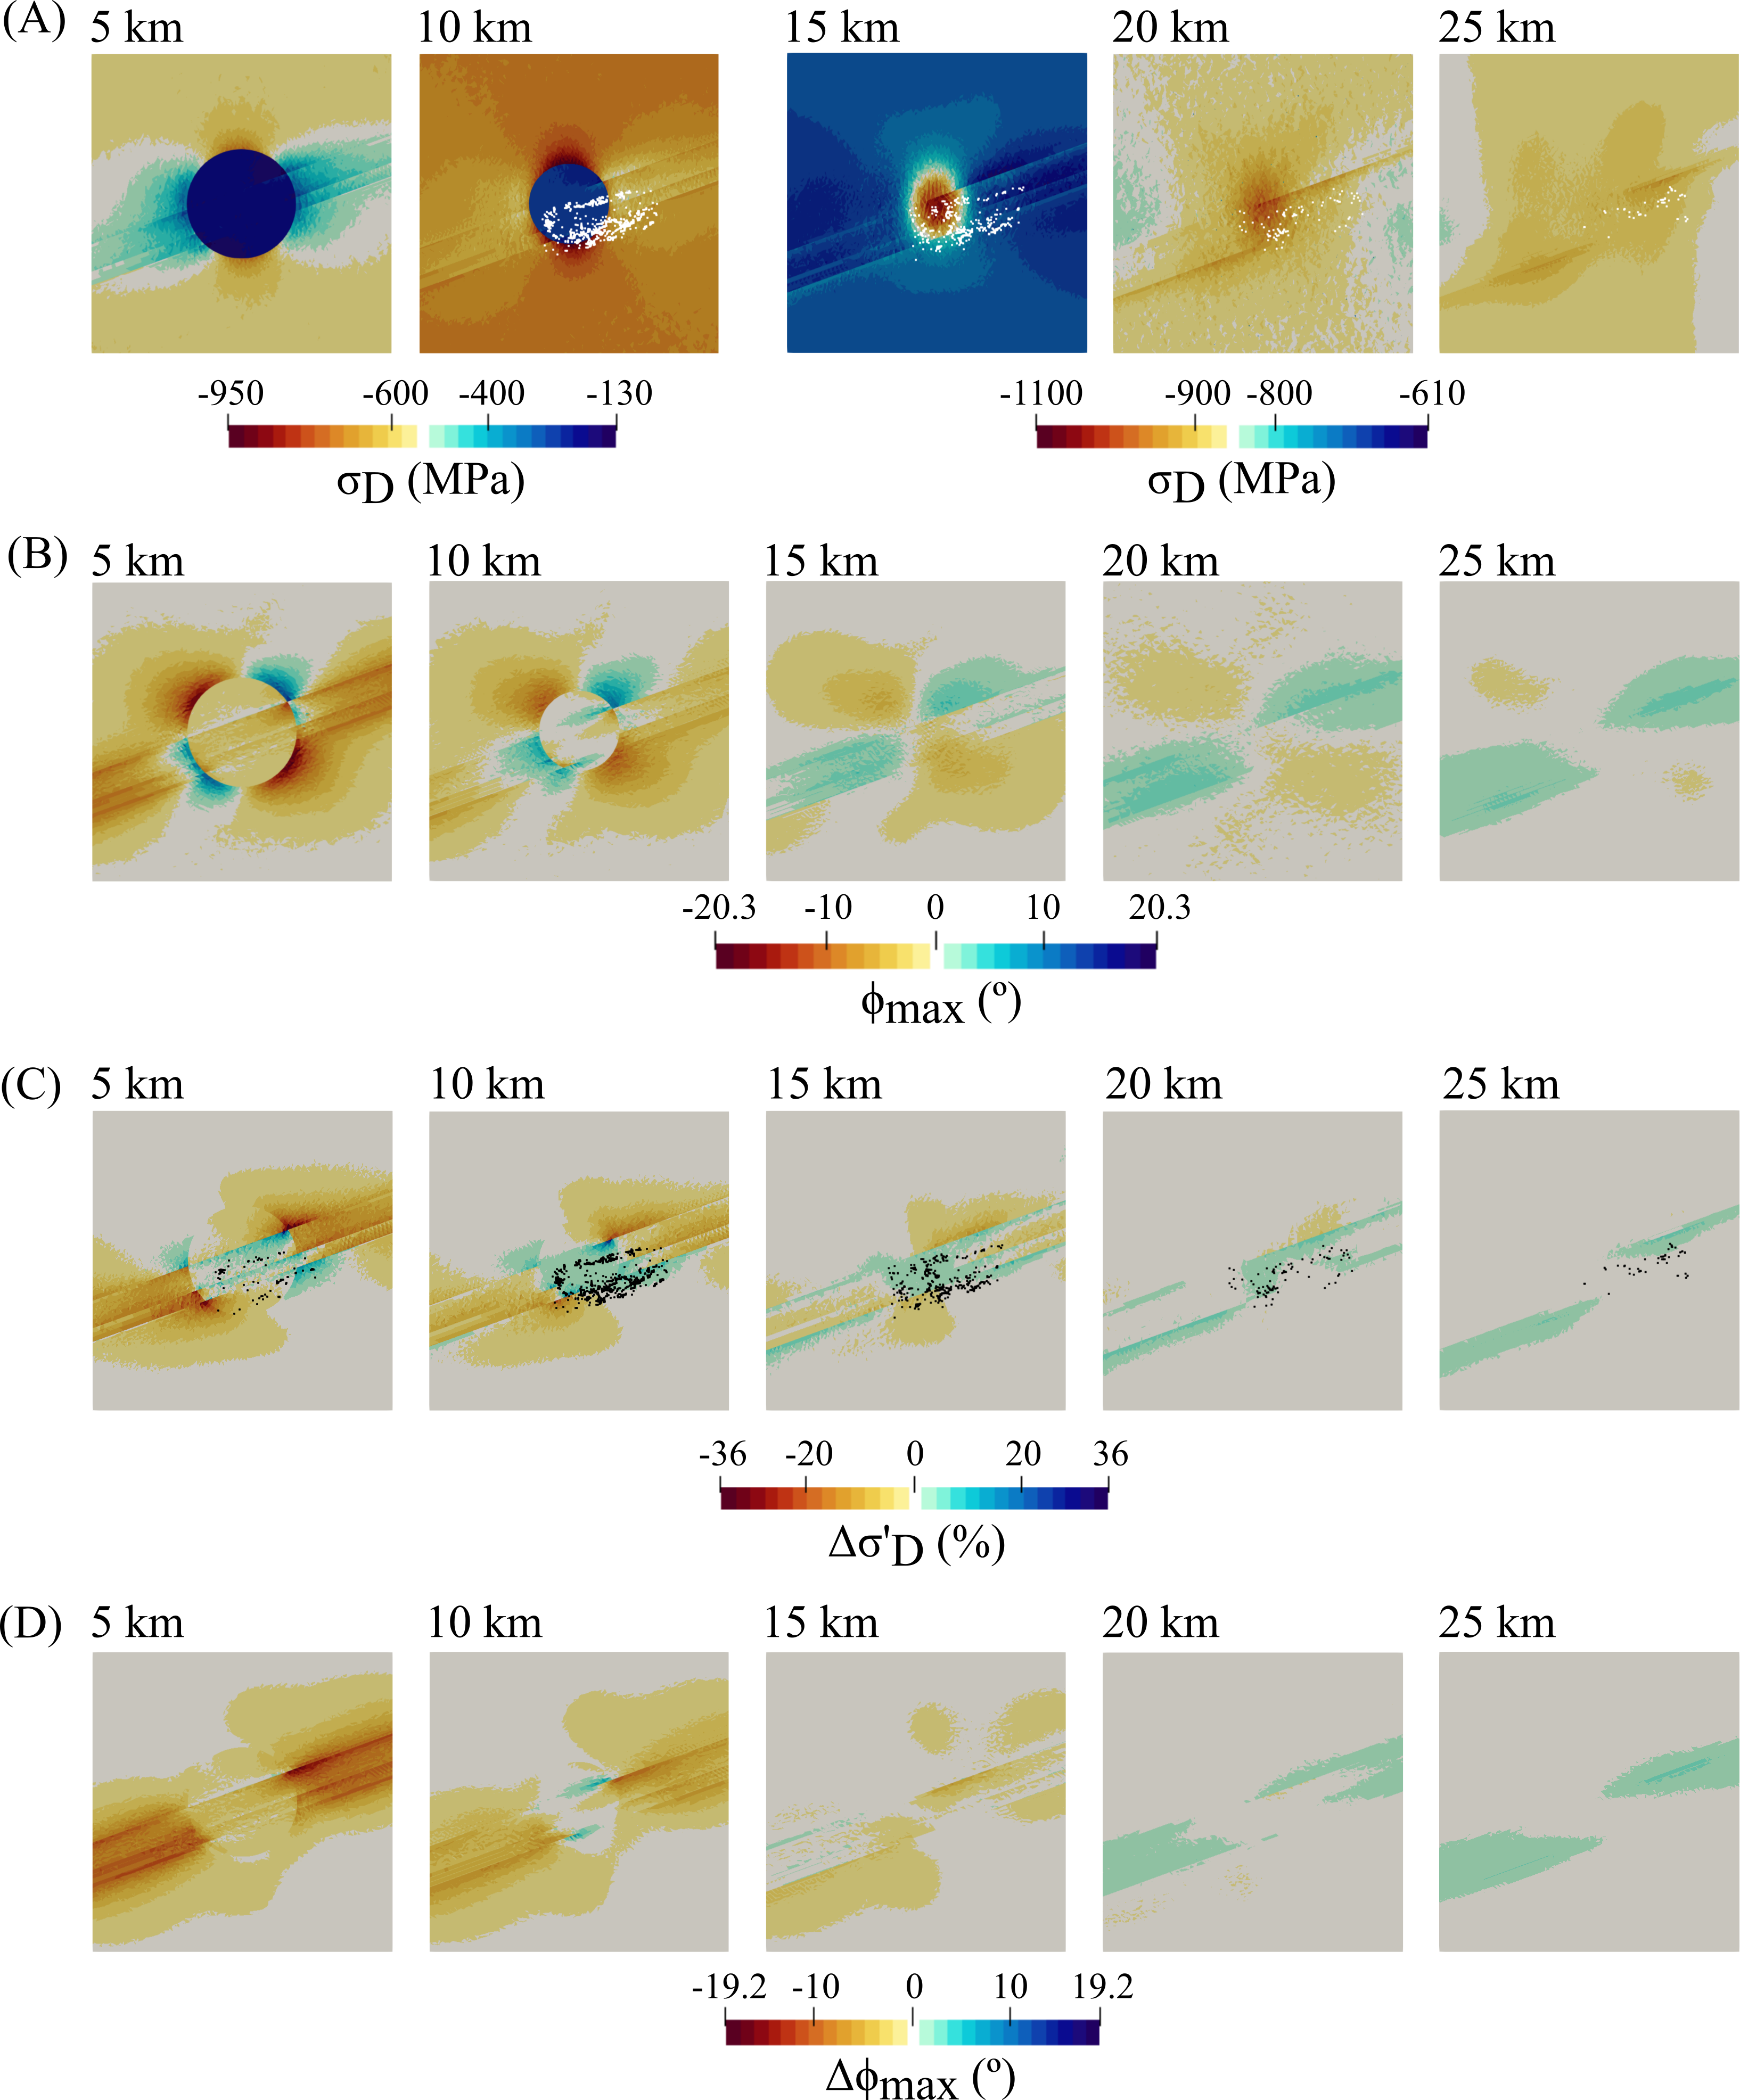
\includegraphics[width=25pc]{Figures/SD70R25.png}
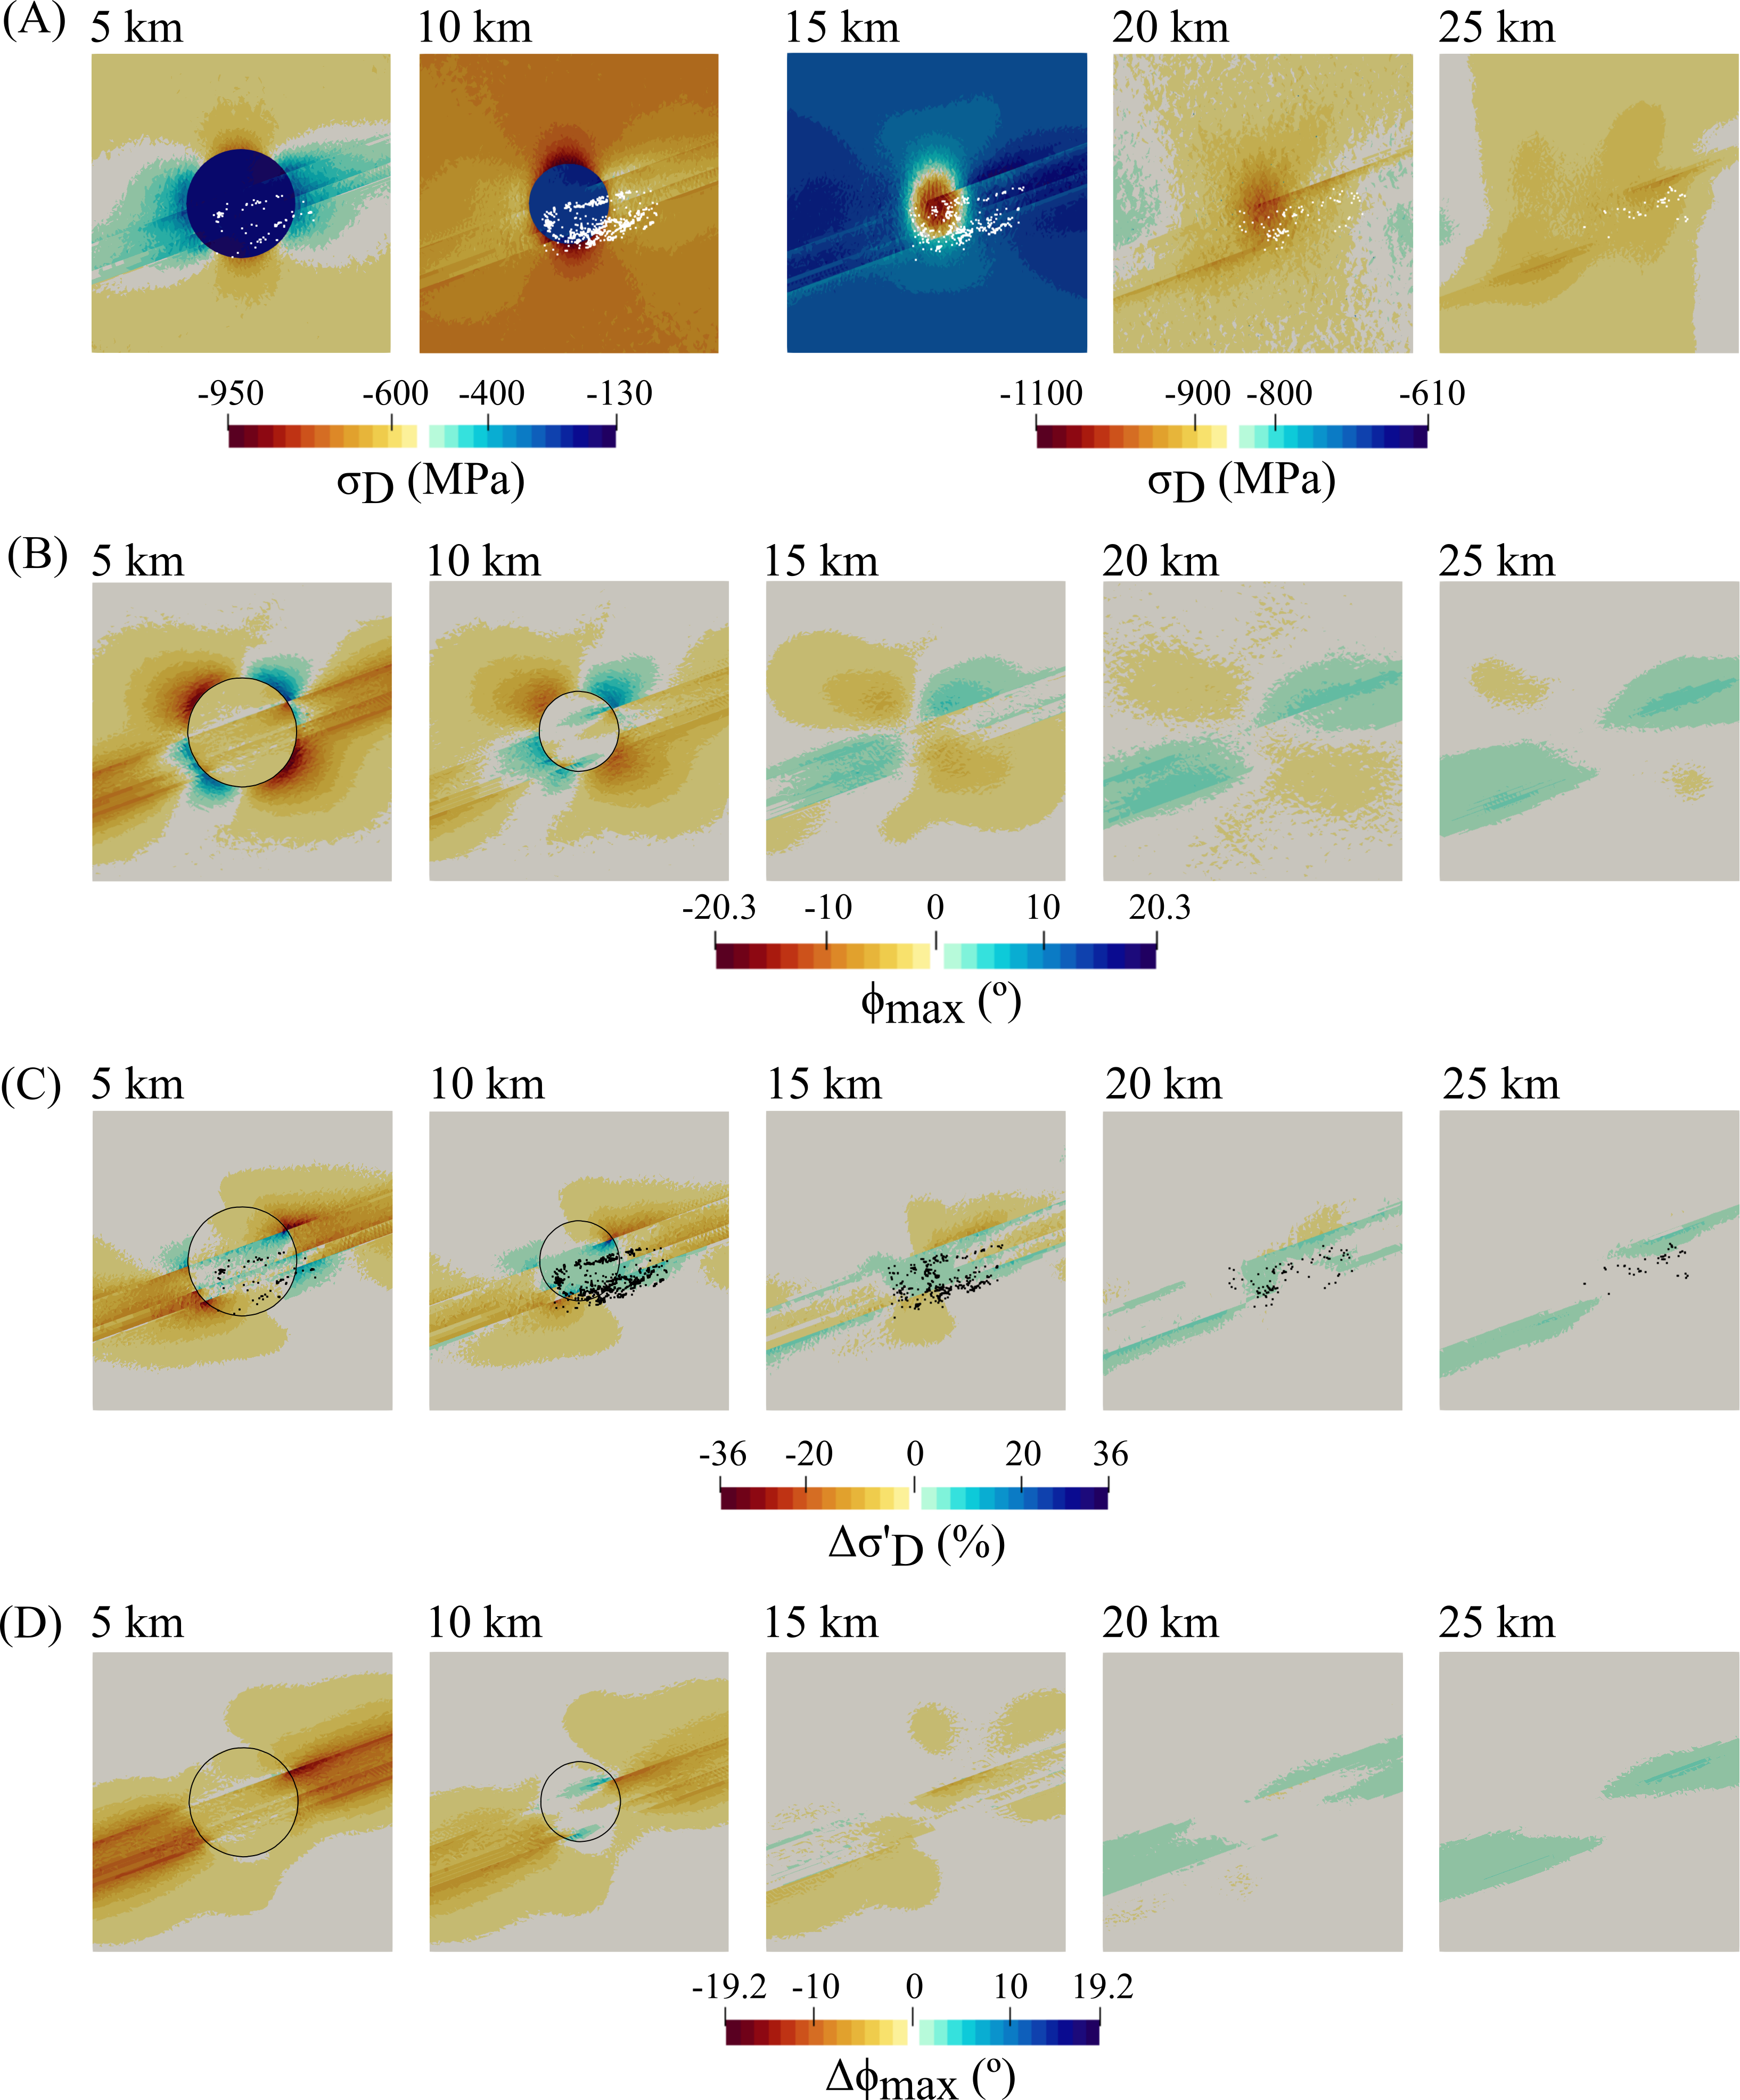
\includegraphics[width=25pc]{SD70R25_2.png}
\caption{(A) Differential stress ($\sigma_D$), (B) SH$_{\max}$ orientation ($\phi_{\max}$), (C) Percentage change in differential stress  ($\Delta\sigma_{D}^{\prime}$) and (D) the change in $\phi_{\max}$ ($\Delta\phi_{\max}$) in SD70R25 model relative to SNFR25 at various depths. Note the change in scale in \ref{fig:SD70R25}A for depths greater than 10 km. Earthquakes within 2 km of each depth slice are represented by black dots in \ref{fig:SD70R25}C. \add[OF]{The outline of the impact structure is represented as a black circle.} Each figure is 70 $\times$ 70 km.} 
\label{fig:SD70R25}
\end{figure}

$\phi_{\max}$ shows a four-lobe pattern of alternating polarities around the weaker \change[OF]{crater}{impact structure} but modifications made by the faults are also clearly visible. $\phi_{\max}$ in the surrounding crust approaches 0$^\circ$ as distance from the \change[OF]{crater}{impact structure}'s center or depth increases (Fig. \ref{fig:SD70R25}B). $\phi_{\max}$ within the \change[OF]{crater}{impact structure} is about $-5^{\circ}$ at a depth of 5 km but is subparallel to the regional stress orientation at 10 km depth (Fig. \ref{fig:SD70R25}B). The main effect of the rift faults is a 5$^{\circ}$ to 15$^{\circ}$ $\phi_{\max}$ clockwise rotation that persists along the faults at 5 and 10 km depths. The sense of near-fault $\phi_{\max}$ rotations flips to anticlockwise at 10 km within the \change[OF]{crater}{impact structure} and at depths below the \change[OF]{crater}{impact structure} in the surrounding crust. The anticlockwise rotation also persists along the faults and has a magnitude of about 5$^{\circ}$.

The distribution of positive $\Delta\sigma_{D}^{\prime}$ values, corresponding to increased differential stresses in SD70R25 relative to SNFR25, spatially overlaps with the seismicity in general and particularly well at 10 km (Fig. \ref{fig:SD70R25}C). \add[OF]{About 70\% of the hypocenters fall in the region with $\Delta\sigma_{D}^{\prime} \ge$ 0.5\%.} We superimpose the relocated hypocenters of earthquakes of \citet{Powell_2017} that occurred within 2 km of each depth slice. The hypocenters are rotated clockwise by 35$^{\circ}$ about the center of the \change[OF]{crater}{impact structure} in order for them to be consistent with the rotated model geometry. Some earthquakes fall in the region of negative $\Delta\sigma_{D}^{\prime}$ near the SW and NE boundary of the \change[OF]{crater}{impact structure} at depths shallower than 15 km.

The $\Delta\phi_{\max}$ maps in Fig. \ref{fig:SD70R25}D show that the rift faults rotate SH$_{\max}$ of SNFR25 further clockwise at 5 and 10 km depths by up to 19$^{\circ}$. The effect of clockwise rotation due to the faults is diminished within the \change[OF]{crater}{impact structure} and flips the sense of rotation to anticlockwise at 10 km (Fig. \ref{fig:SD70R25}D). At depths below the \change[OF]{crater}{impact structure}, the overall impact of the faults decrease everywhere.

Three vertical cross sections of $\Delta\sigma_{D}^{\prime}$ from the SD70R25 model are shown in Fig.~\ref{fig:profiles_70_70_70_2km}. As marked on the 10-km depth slice of $\Delta\sigma_{D}^{\prime}$ (left panel in Fig.~\ref{fig:profiles_70_70_70_2km}), they are all perpendicular to the fault strike. Two cross sections, 1 and 2, go through the central and marginal areas of the \change[OF]{crater}{impact structure} but the cross section 3 does not intersect the \change[OF]{crater}{impact structure}. Also plotted on these cross sections are the hypocenters of the region's earthquakes within 2 km from each cross section. Most of the earthquakes fall within regions of increased differential stress but some are associated with negative or negligible changes in differential stress. In the cross sections going through the \change[OF]{crater}{impact structure}, the broad region between the northernmost and the southernmost fault shows positive $\Delta\sigma_{D}^{\prime}$. In contrast, the relocated hypocenters exhibit well-defined linear trends as observed by~\citet{Powell_2017}.

\begin{figure}[ht]
\centering
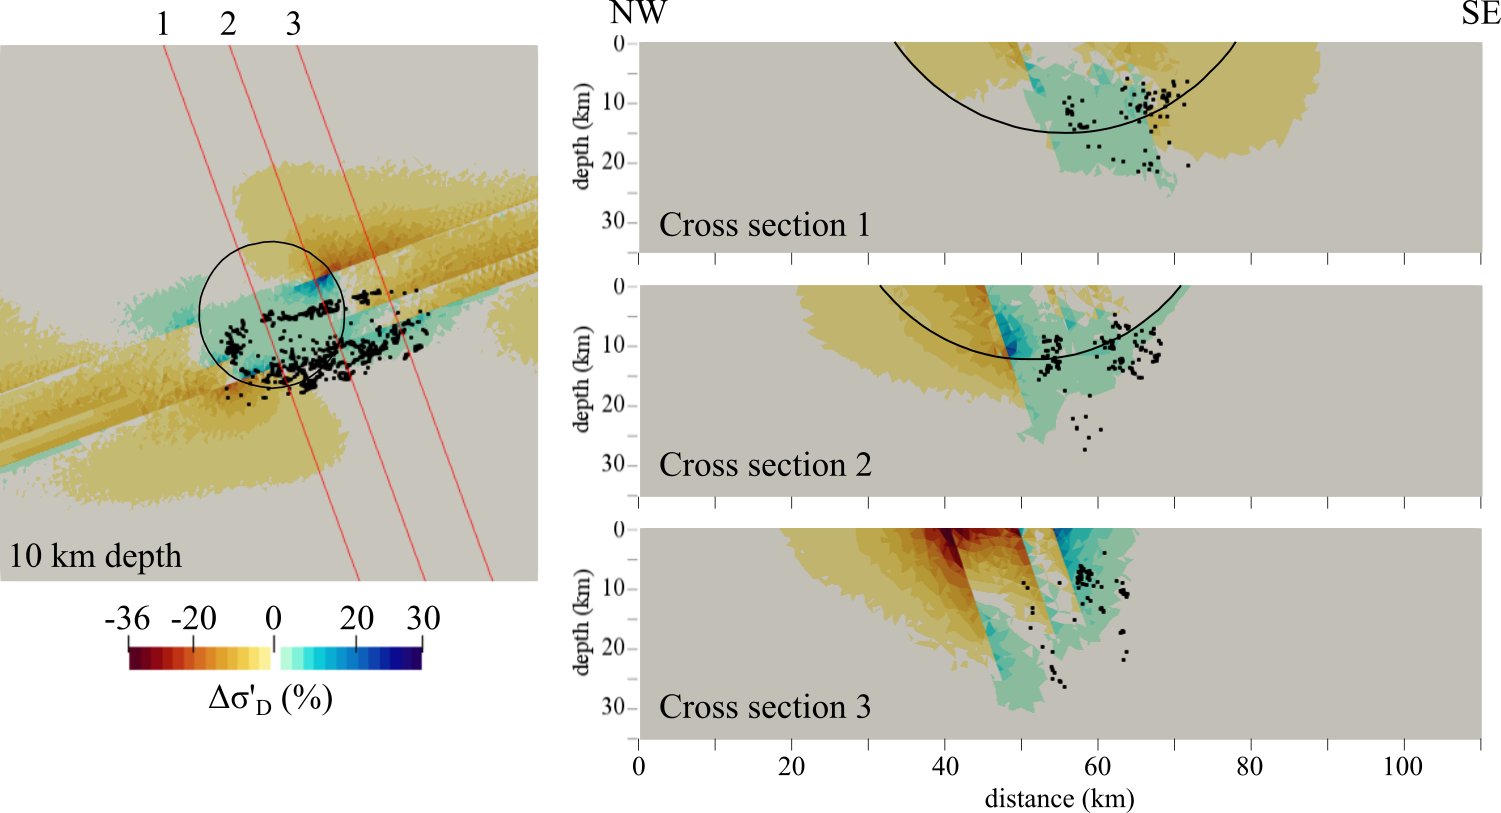
\includegraphics[width=25pc]{SD70R25_profiles.png}
\caption{NW-SE cross sections through the percentage change in differential stress ($\Delta\sigma_{D}^{\prime}$) solution in the SD70R25 model. Earthquakes within 2 km of each cross section are represented by black dots. The three NW-SE cross sections are indicated on the 10-km depth slice showing earthquakes within 2 km of the depth slice. The outline of the \change[OF]{crater}{impact structure} is represented as black circle and curved lines on the depth slice and cross sections, respectively. The depth slice is 70 $\times$ 70 km centered on the impact \change[OF]{crater}{structure}. Note the cross sections have the same color and length scales as the depth slice in~\ref{fig:profiles_70_70_70_2km}A.}
\label{fig:profiles_70_70_70_2km}
\end{figure}

% #############################################################

\subsubsection{SD65R25}
Correlation between the $\Delta\sigma_{D}^{\prime}$ distribution in SD65R25 and the observed seismicity is not as clear as in SD70R25 but shows more fine-scale correlation with the observed seismicity, especially at 10 km depth (Fig. \ref{fig:eff_of_dips}). At 15 km depth, the region of positive $\Delta\sigma_{D}^{\prime}$ correlates with the earthquakes on the northernmost fault but the earthquakes on the middle rift fault fall in regions with negative $\Delta\sigma_{D}^{\prime}$. 

\begin{figure}[ht]
\centering
%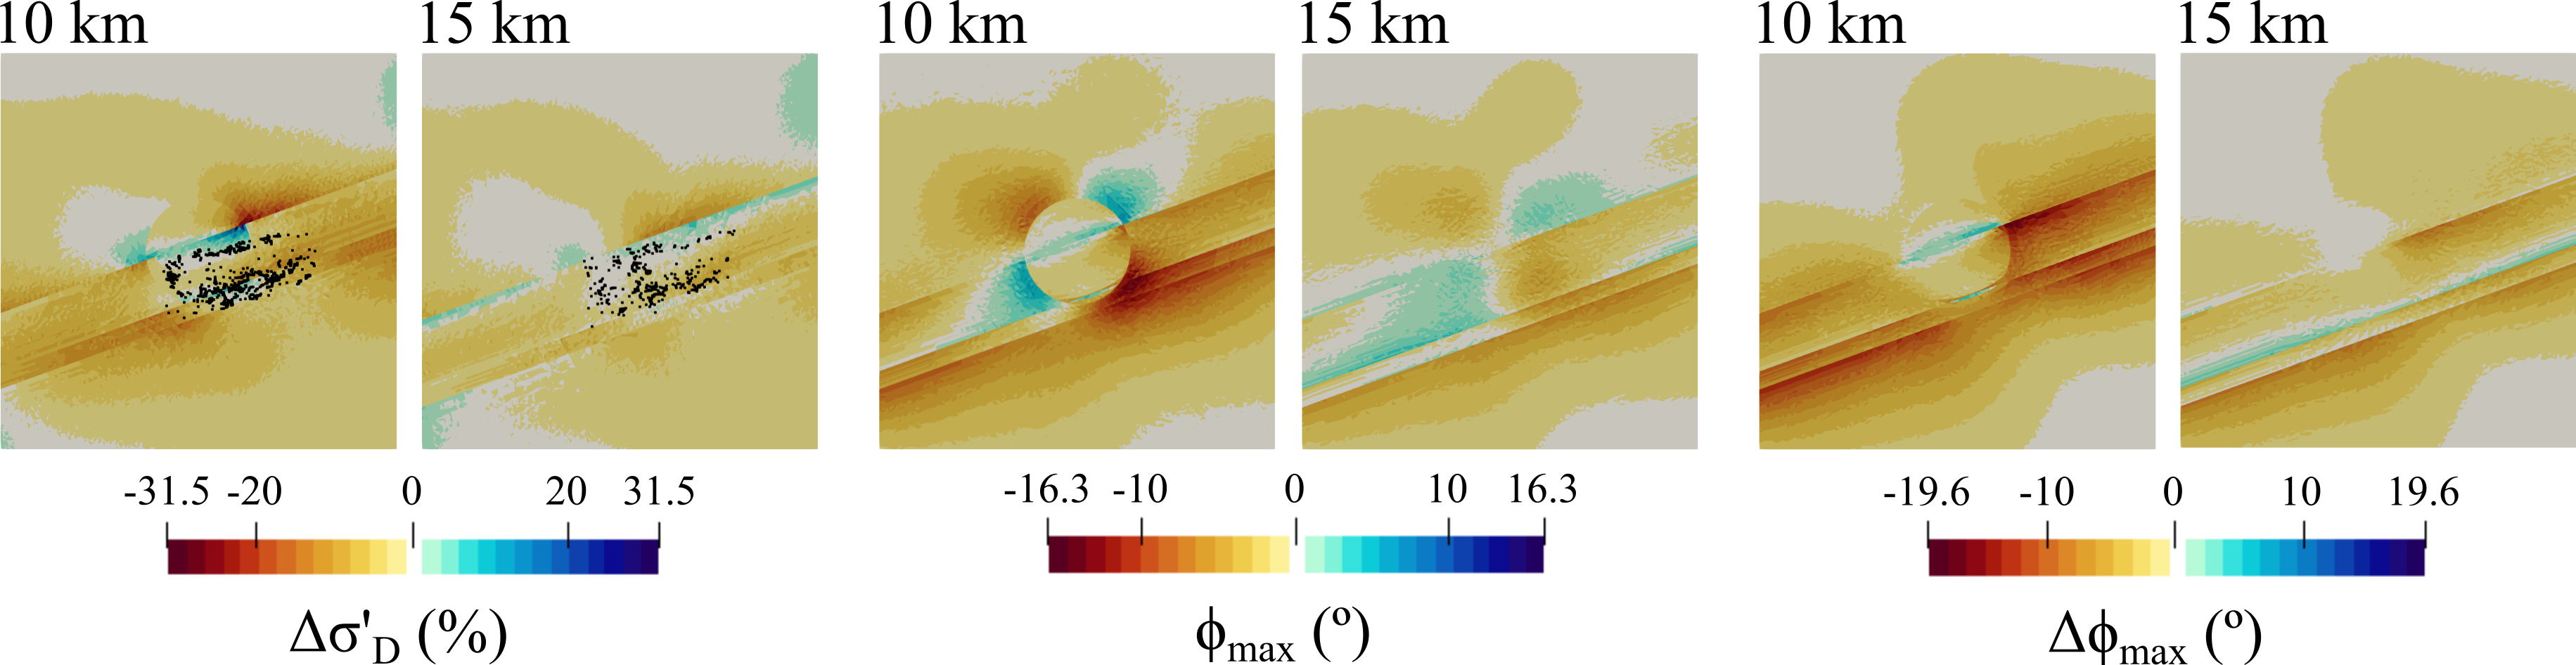
\includegraphics[width=30pc]{Figures/SD65R25.png}
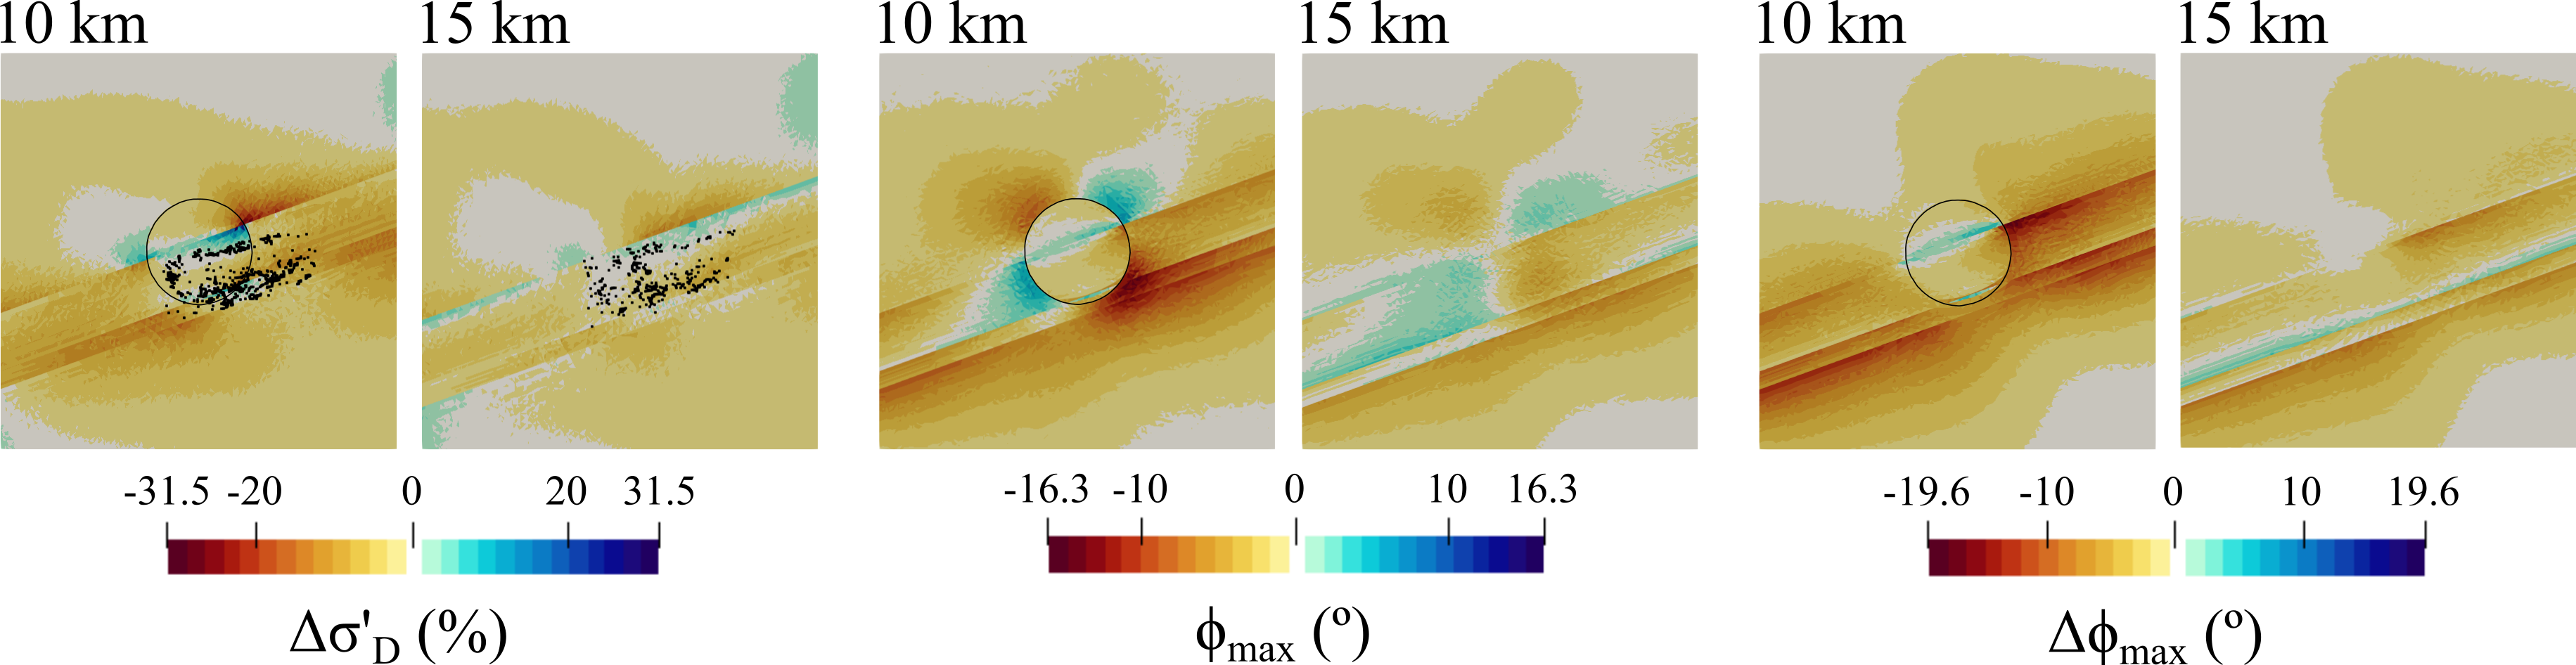
\includegraphics[width=30pc]{SD65R25_2.png}
\caption{Percentage change in differential stress ($\Delta\sigma_{D}^{\prime}$), SH$_{\max}$ orientation ($\phi_{\max})$ and the change in $\phi_{\max}$ ($\Delta\phi_{\max}$) at 10 and 15 km depths from the SD65R25 model. Earthquakes within 2 km of each depth slice are represented by black dots in \ref{fig:eff_of_dips}A. \add[OF]{The outline of the impact structure is represented as a black circle.} Each figure is 70 $\times$ 70 km.}
\label{fig:eff_of_dips}
\end{figure}

Greater clockwise rotations of SH$_{\max}$ are found in SD65R25 than in SD70R25 at all depths (Fig. \ref{fig:eff_of_dips}) although both models show the four-lobe pattern and magnitudes of $\phi_{\max}$ decreasing with depth. Within the \change[OF]{crater}{impact structure}, SD65R25 shows clockwise rotations of about 5$^\circ$ at 10 km depth and the counterclockwise rotation observed for model SD70R25 is seen only north of the northernmost fault because the other two faults barely cross the \change[OF]{crater}{impact structure} region at this depth due to their shallower dip (Fig. \ref{fig:eff_of_dips}). In the surrounding crust close to the rift faults, $\phi_{\max}$ rotates clockwise by 5$^\circ$ to 16.3$^\circ$ relative to the regional stress direction (Fig. \ref{fig:eff_of_dips}). Counterclockwise rotation of $\phi_{\max}$ relative to the regional SH$_{\max}$ extends to the northeast and southwest of the \change[OF]{crater}{impact structure} in the fault-bounded region.

When compared to SH$_{\max}$ orientations in the reference model, SD65R25 shows greater clockwise rotations of $\phi_{\max}$ by up to 20$^\circ$ near the rift faults and the northeastern boundary of the \change[OF]{crater}{impact structure} at 10 km depth (Fig. \ref{fig:eff_of_dips}). These values of $\Delta \phi_{\max}$ are greater than those of SD70R25 and thus can be attributed to the shallower dips of the faults in SD65R25.

The region of increased differential stress in SD65R25 exhibits well-defined linear trends near the rift faults, and thus gives a better explanation for the narrow and well-defined seismicity near the \change[OF]{crater}{impact structure} (Fig. \ref{fig:profiles_65_40_40_2km}). \add[OF]{About 25\% of the hypocenters fall in the region with $\Delta\sigma_{D}^{\prime} \ge$ 0.5\%.}. The SD65R25 model shows a region of negative $\Delta\sigma_{D}^{\prime}$ between the observed seismicity on the northernmost and southernmost faults. The earthquakes on the middle rift fault and most of the earthquakes on the southernmost fault outside the \change[OF]{crater}{impact structure} fall in regions with negative $\Delta\sigma_{D}^{\prime}$ (Fig. \ref{fig:profiles_65_40_40_2km}).

%\note[EC]{Why do you say ``even though''? Does the percentage betray your or a general expectation?} \add[OF]{, even though the overall percentage of the hypocenters that fall in region with $\Delta\sigma_{D}^{\prime} \ge$ 0.5\% is about 25\%.}

\begin{figure}[ht]
\centering
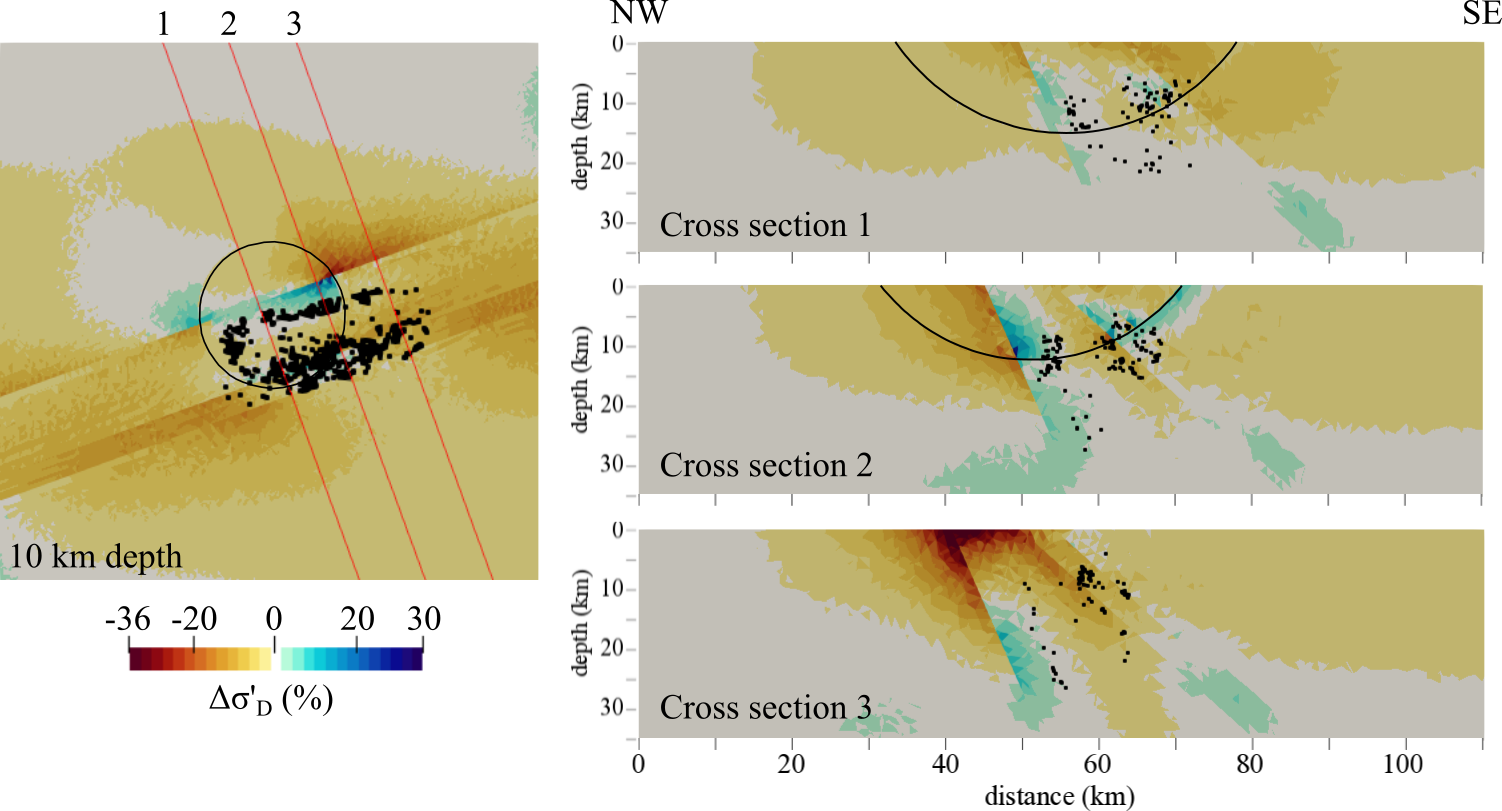
\includegraphics[width=25pc]{SD65R25_profiles.png}
\caption{Same as Fig. \ref{fig:profiles_70_70_70_2km} but for SD65R25 model.}
\label{fig:profiles_65_40_40_2km}
\end{figure}

\subsection{Effects of the weakness of the damaged \change[OF]{crater}{impact structure} zone}
Two models with the rift faults dipping at 70$^{\circ}$ are constructed such that the ratio of elastic moduli of the \change[OF]{crater}{impact structure} to that of the surrounding crust are 0.5 (SD70R50) and 1.0 (SD70R100), respectively.

\subsubsection{SD70R50}
While the effects of the \change[OF]{crater}{impact structure} and rift faults are still clear and consistent, SD70R50 values of $\Delta \sigma_{D}^{\prime}$ are mostly negative with some exceptions at 10 km depth amounting to about a 10 \% increased stress (Fig. \ref{fig:eff_of_moduli_ratio}A). The region of positive $\Delta\sigma_{D}^{\prime}$ in the SD70R50 model overlaps with the hypocenters only in the southeast corner of the \change[OF]{crater}{impact structure} boundary and the southernmost rift fault (i.e., the Charlevoix fault) at 5 km depth \add[OF]{, amounting to about 45\% of the hypocenters in the region with $\Delta\sigma_{D}^{\prime} \ge$ 0.5\%.} (Fig. \ref{fig:eff_of_moduli_ratio}A). The spatial correlation of seismicity with increased $\sigma_{D}$ relative to the reference model is stronger at 10 km depth.

\begin{figure}[ht]
\centering
%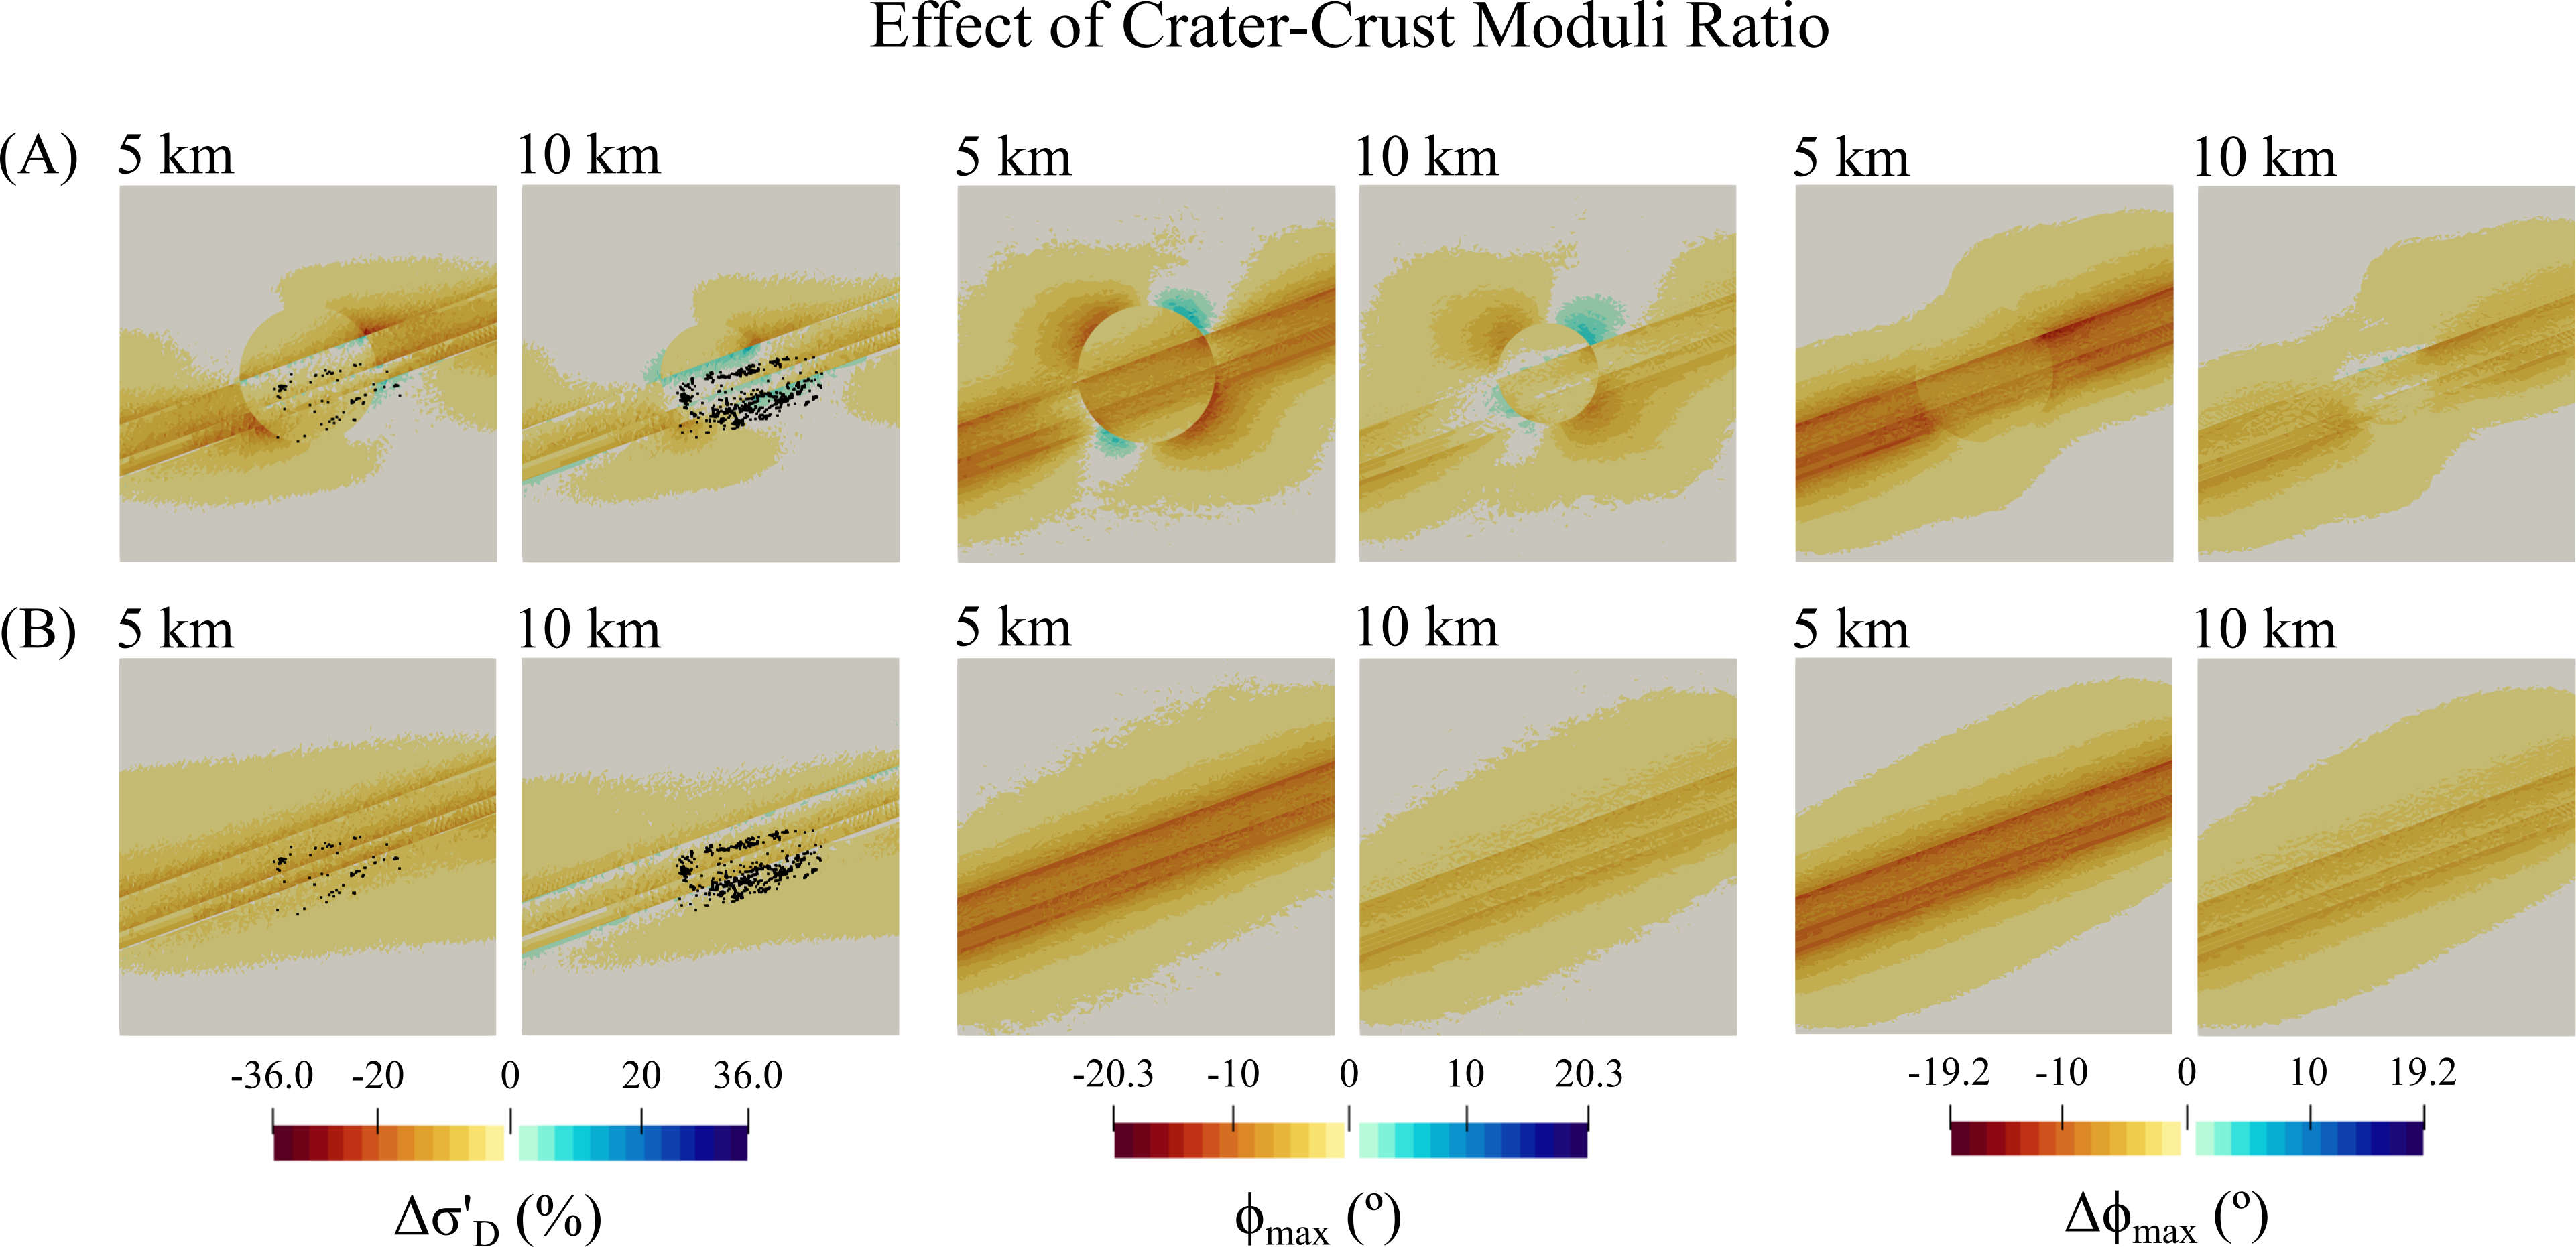
\includegraphics[width=30pc]{Figures/SD70R50_100.png}
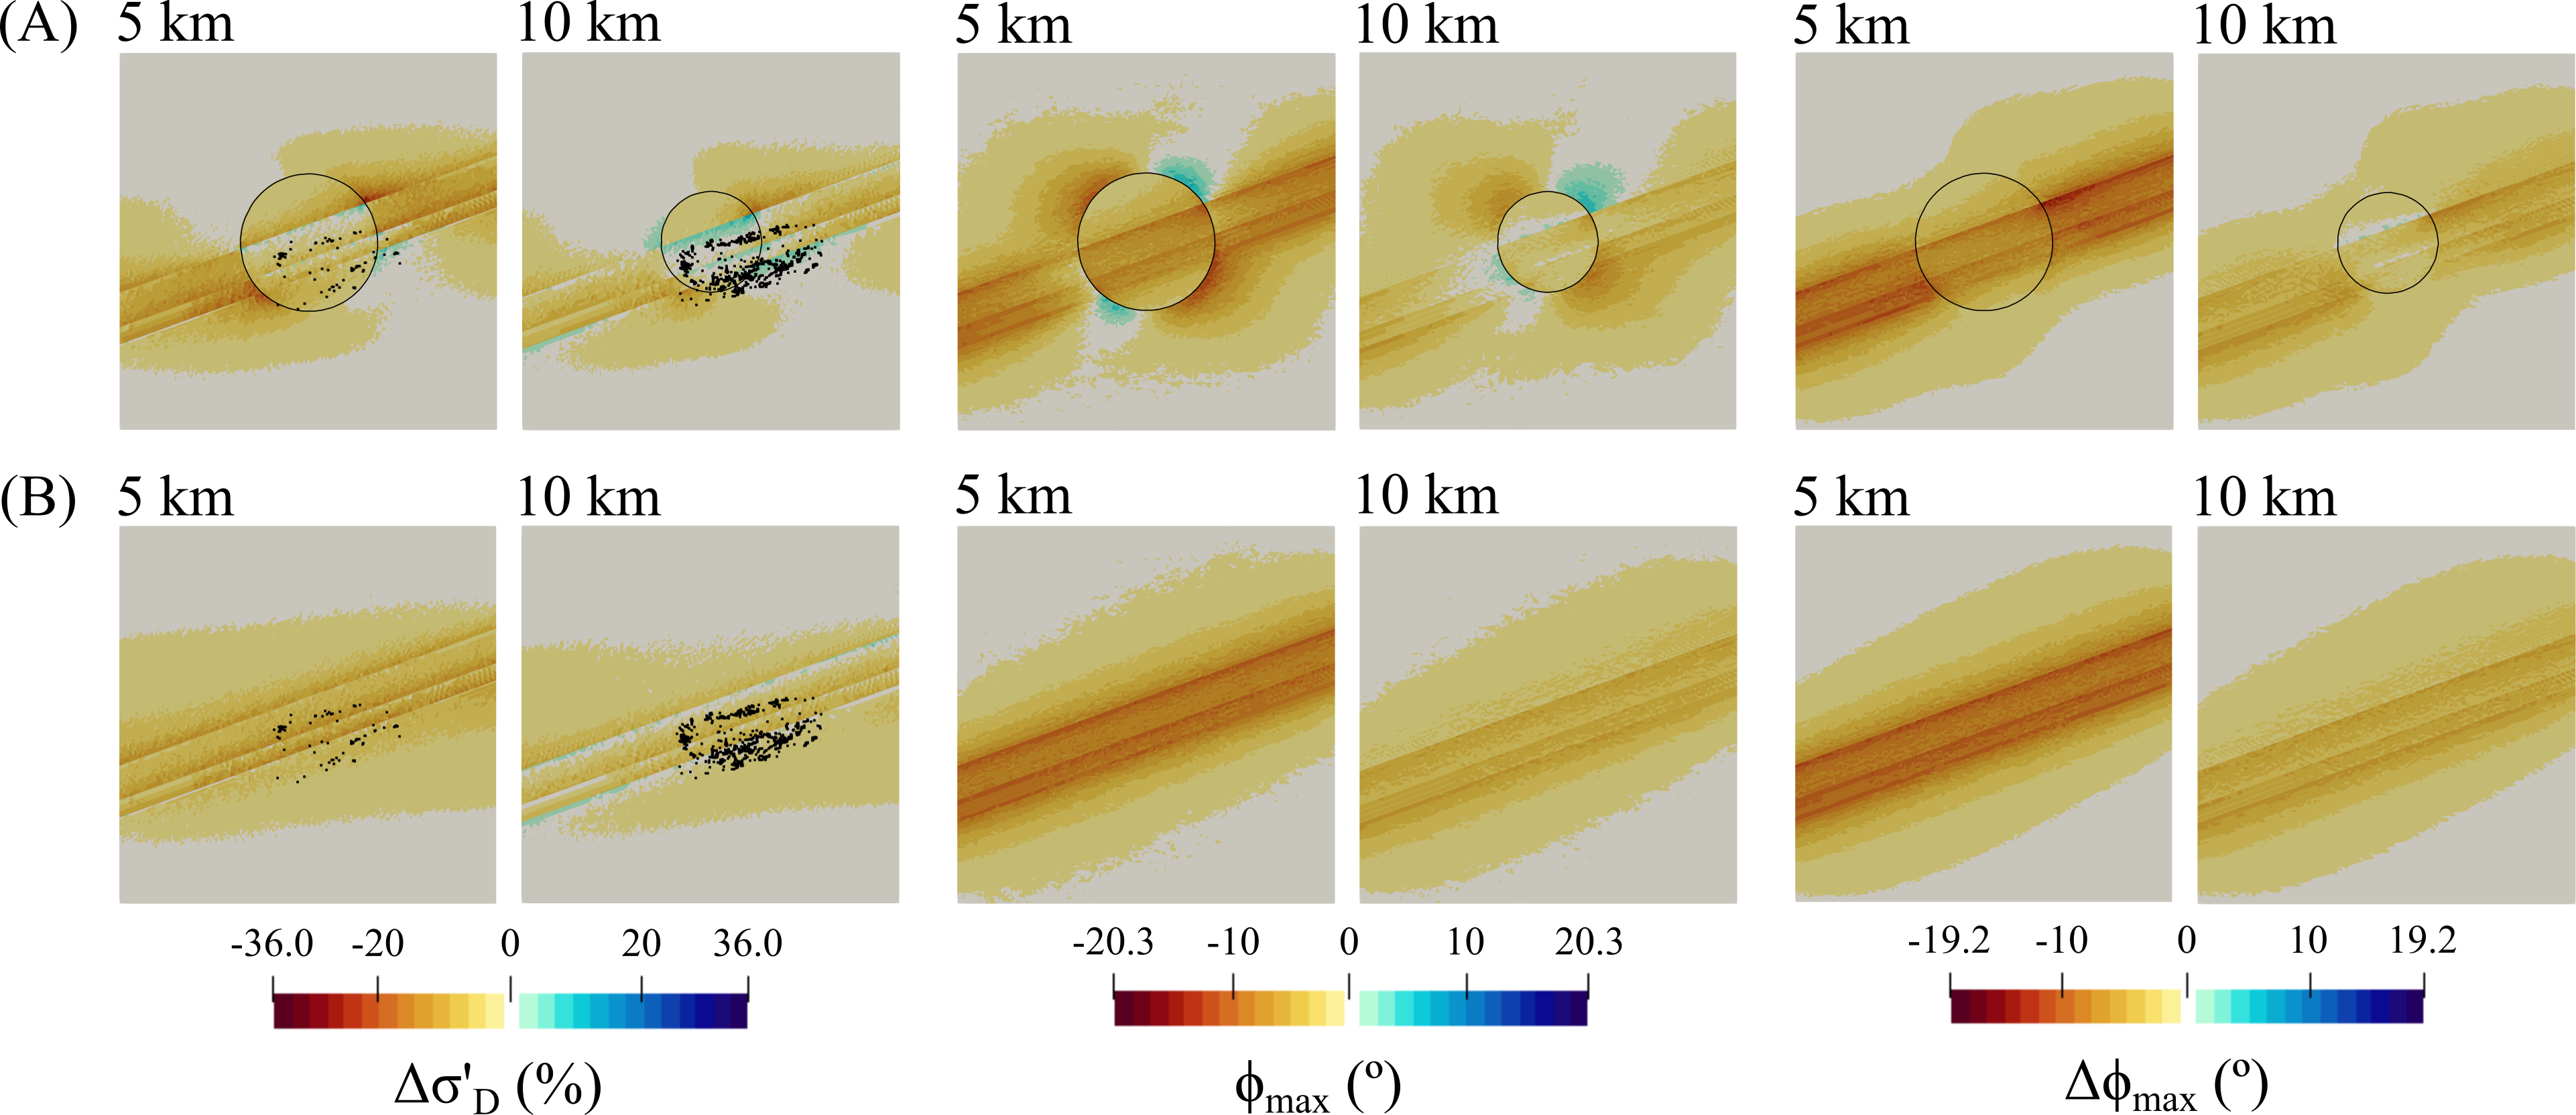
\includegraphics[width=30pc]{SD70R50_100_2.png}
\caption{Same as Fig.~\ref{fig:eff_of_dips} but for the models with different \change[OF]{crater}{impact structure}-crust elastic moduli ratios: (A) SD70R50 and (B) SD70R100.}
\label{fig:eff_of_moduli_ratio}
\end{figure}

$\phi_{\max}$ plots show the four-lobe pattern of alternating polarities and shows the effects of the rift faults. The maximum value of $\phi_{\max}$ is about 13$^\circ$ (Fig. \ref{fig:eff_of_moduli_ratio}A). The $\Delta\phi_{\max}$ maps in Fig. \ref{fig:eff_of_moduli_ratio}A show that the rift faults rotates the $\phi_{\max}$ in the reference model at 5 and 10 km depths up to 16.5$^{\circ}$. The value of $\Delta\phi_{\max}$ decreases to almost zero at 15 km depth, and is anticlockwise up to $-3^{\circ}$ at 20 and 25 km depths.

% #############################################################
\subsubsection{SD70R100}
$\Delta\sigma_{D}^{\prime}$ and $\phi_{\max}$ only exhibit the effects of the rift faults since the \change[OF]{crater}{impact structure} and the crust have the same elastic moduli in model SD70R100 (Fig. \ref{fig:eff_of_moduli_ratio}B).

Positive $\Delta\sigma_{D}^{\prime}$ values in SD70R100 are seen only at a depth of 10 km and their distribution does not fit the observed seismicity (Fig. \ref{fig:eff_of_moduli_ratio}B).  \add[OF]{About 23\% of the hypocenters fall in the region with $\Delta\sigma_{D}^{\prime} \ge$ 0.5\%.} $\Delta\sigma_{D}^{\prime}$ correlates with observed seismicity below 15 km except for some earthquakes in the northern cluster. However, the model predicts earthquakes throughout the entire length of the rift faults at and below 15 km depth. Figures that shows all the depth slices are in the supplementary materials (Fig. S4). \add[OF]{The result of a model with an intermediate moduli ratio of 0.75 is somewhat between the SD70R50 and SD70R100 models (Fig. S5).}

The distribution of $\phi_{\max}$ values lacks the four-lobe pattern and is negative in the vicinity of the rift faults at 5 and 10 km depth: i.e., $\phi_{\max}$ values are rotated clockwise relative to the regional SH$_{\max}$ (Fig. \ref{fig:eff_of_moduli_ratio}B). The values of $\phi_{\max}$ range from 2$^\circ$ (25 km depth) to 12.8$^\circ$ (5 km depth). $\phi_{\max}$ decreases to 0$^{\circ}$ at about 50 km from the center of the model along the direction perpendicular to the fault strike.

The maximum value of $\Delta\phi_{\max}$ is 12.8$^\circ$ and, being indistinguishable from $\phi_{\max}$, signifies that the  $\Delta\phi_{\max}$ values in SD70R100 are controlled by the rift faults (Fig. \ref{fig:eff_of_moduli_ratio}B). The value of $\Delta\phi_{\max}$ decreases to almost zero at 15 km depth, and becomes anticlockwise in the fault region at 20 and 25 km.

\subsection{Effects of fault strength (SD70R25V)}
We compute $\sigma_{D}$ and $\phi_{\max}$ in a series of models in which the rift faults dip at 70$^{\circ}$ but their friction coefficient ($\mu$) is varied systematically at a constant cohesion of 0 MPa. We assume that the fault parameters are the same for each rift fault and uniform throughout the fault surfaces. $\mu$ varies from 0.1 to 0.6 with an interval of 0.1. We use a mesh resolution of 4 km for SD70R25V models due to the expensive computation time at $\mu$ values of 0.1 and 0.2. Aside from the change in the friction coefficient and the mesh resolution, the six models computed are the same as SD70R25. $\Delta \sigma_{D}^{\prime}$ and $\phi_{\max}$ computed for these models are plotted in Fig. \ref{fig:eff_of_mu}, which shows 10 km depth sections because of the high number of earthquakes within 2 km from that depth.

Magnitudes of $\Delta \sigma_{D}^{\prime}$ decrease as $\mu$ increases (Fig. \ref{fig:eff_of_mu}A) because the model behaviors must approach those of the no-fault model as fault strength increases. When $\mu$ values are 0.1 and 0.2, the area of positive $\Delta\sigma_{D}^{\prime}$ regions does not cover the entire observed seismicity\add[OF]{, with about 3 and 24\% of the hypocenters within the region of $\Delta\sigma_{D}^{\prime} \ge$ 0.5\%, respectively}. The regions of positive $\Delta\sigma_{D}^{\prime}$ for $\mu$ values equal to 0.3 and 0.4 show better spatial correspondence with the seismicity of the CSZ. However, the model with $\mu = 0.4$ predicts positive Coulomb stress changes along the entire length of the rift faults, which is contrary to the limited spatial extent of the observed seismicity. \add[OF]{Also, about 66\% of the hypocenters in the model with $\mu$ = 0.3 fall within the region of $\Delta\sigma_{D}^{\prime} \ge$ 0.5\% while only 35\% do when $\mu$ = 0.4. However, when the hypocenters falling in the region with $\Delta\sigma_{D}^{\prime} \ge$ 0\% are considered, the percentages increase to 73 and 82\% for $\mu$ equal to 0.3 and 0.4.} 
$\Delta\sigma_{D}^{\prime}$ approaches zero when $\mu$ values are 0.5 and 0.6, for which the faults are locked. \add[OF]{The percentage of hypocenters in the region with $\Delta\sigma_{D}^{\prime} \ge$ 0.5\% reduces to 1.4\% and 0\% when $\mu$ values are 0.5 and 0.6, respectively.}

\begin{figure}[ht]
\centering
%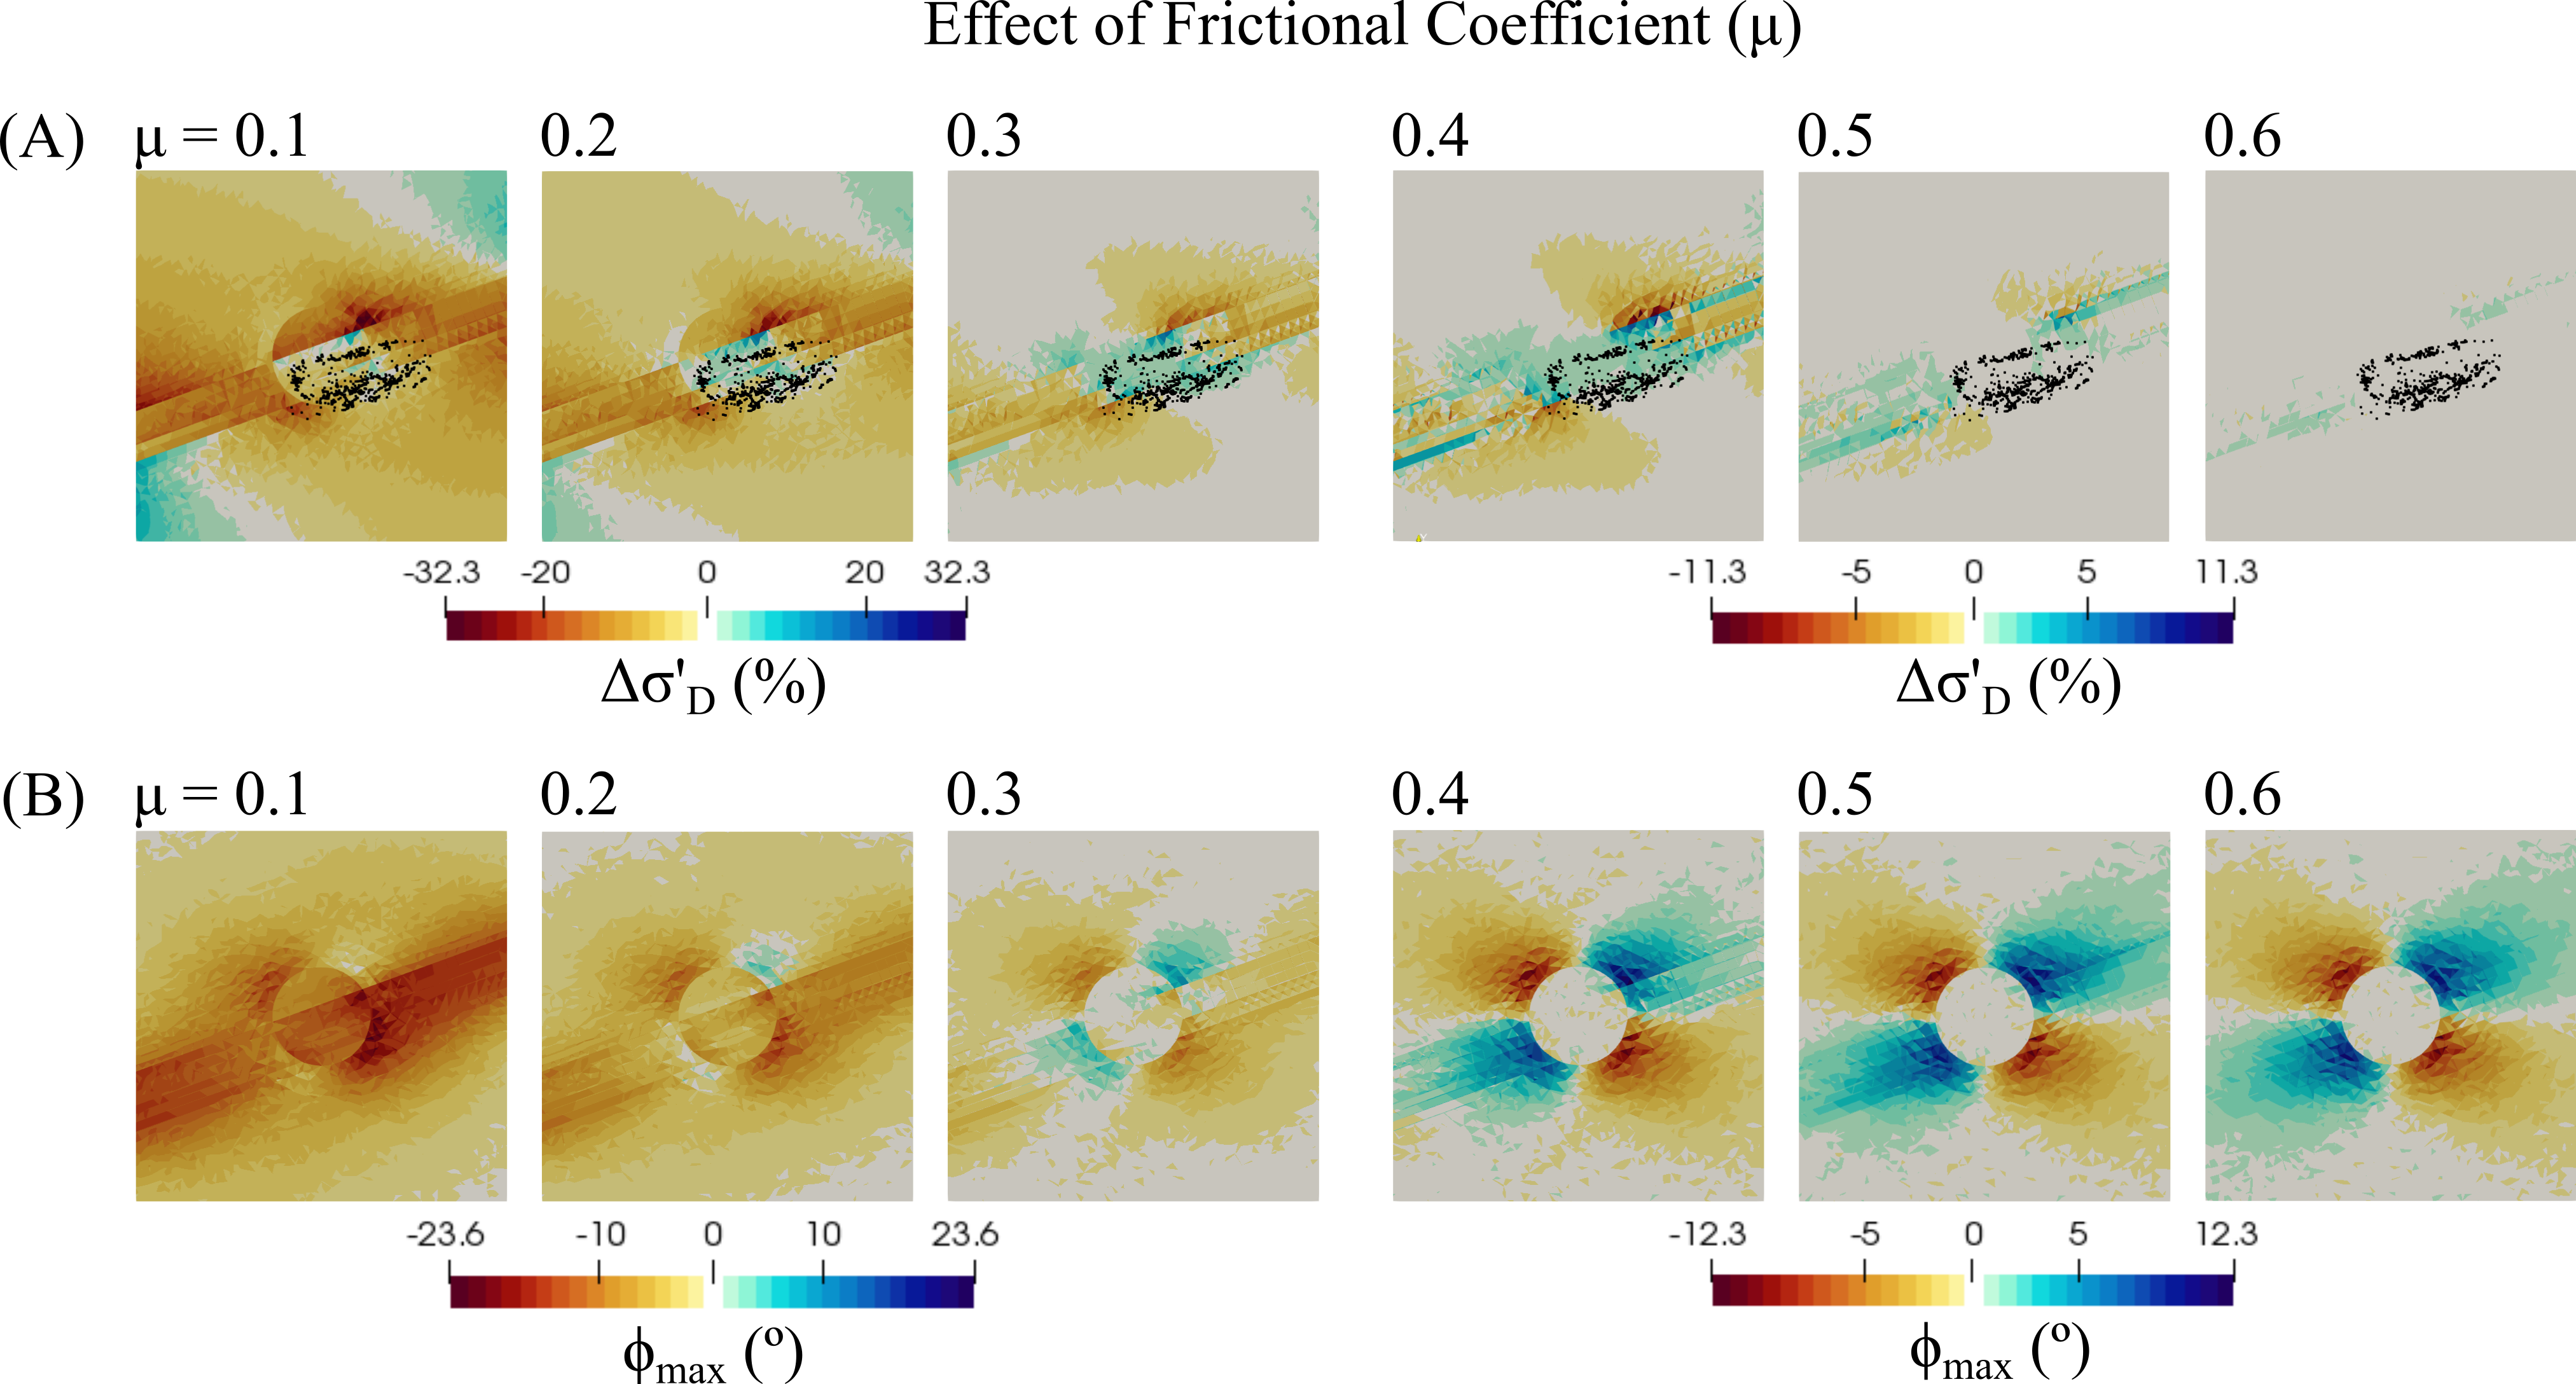
\includegraphics[width=30pc]{Figures/SD70R25V.png}
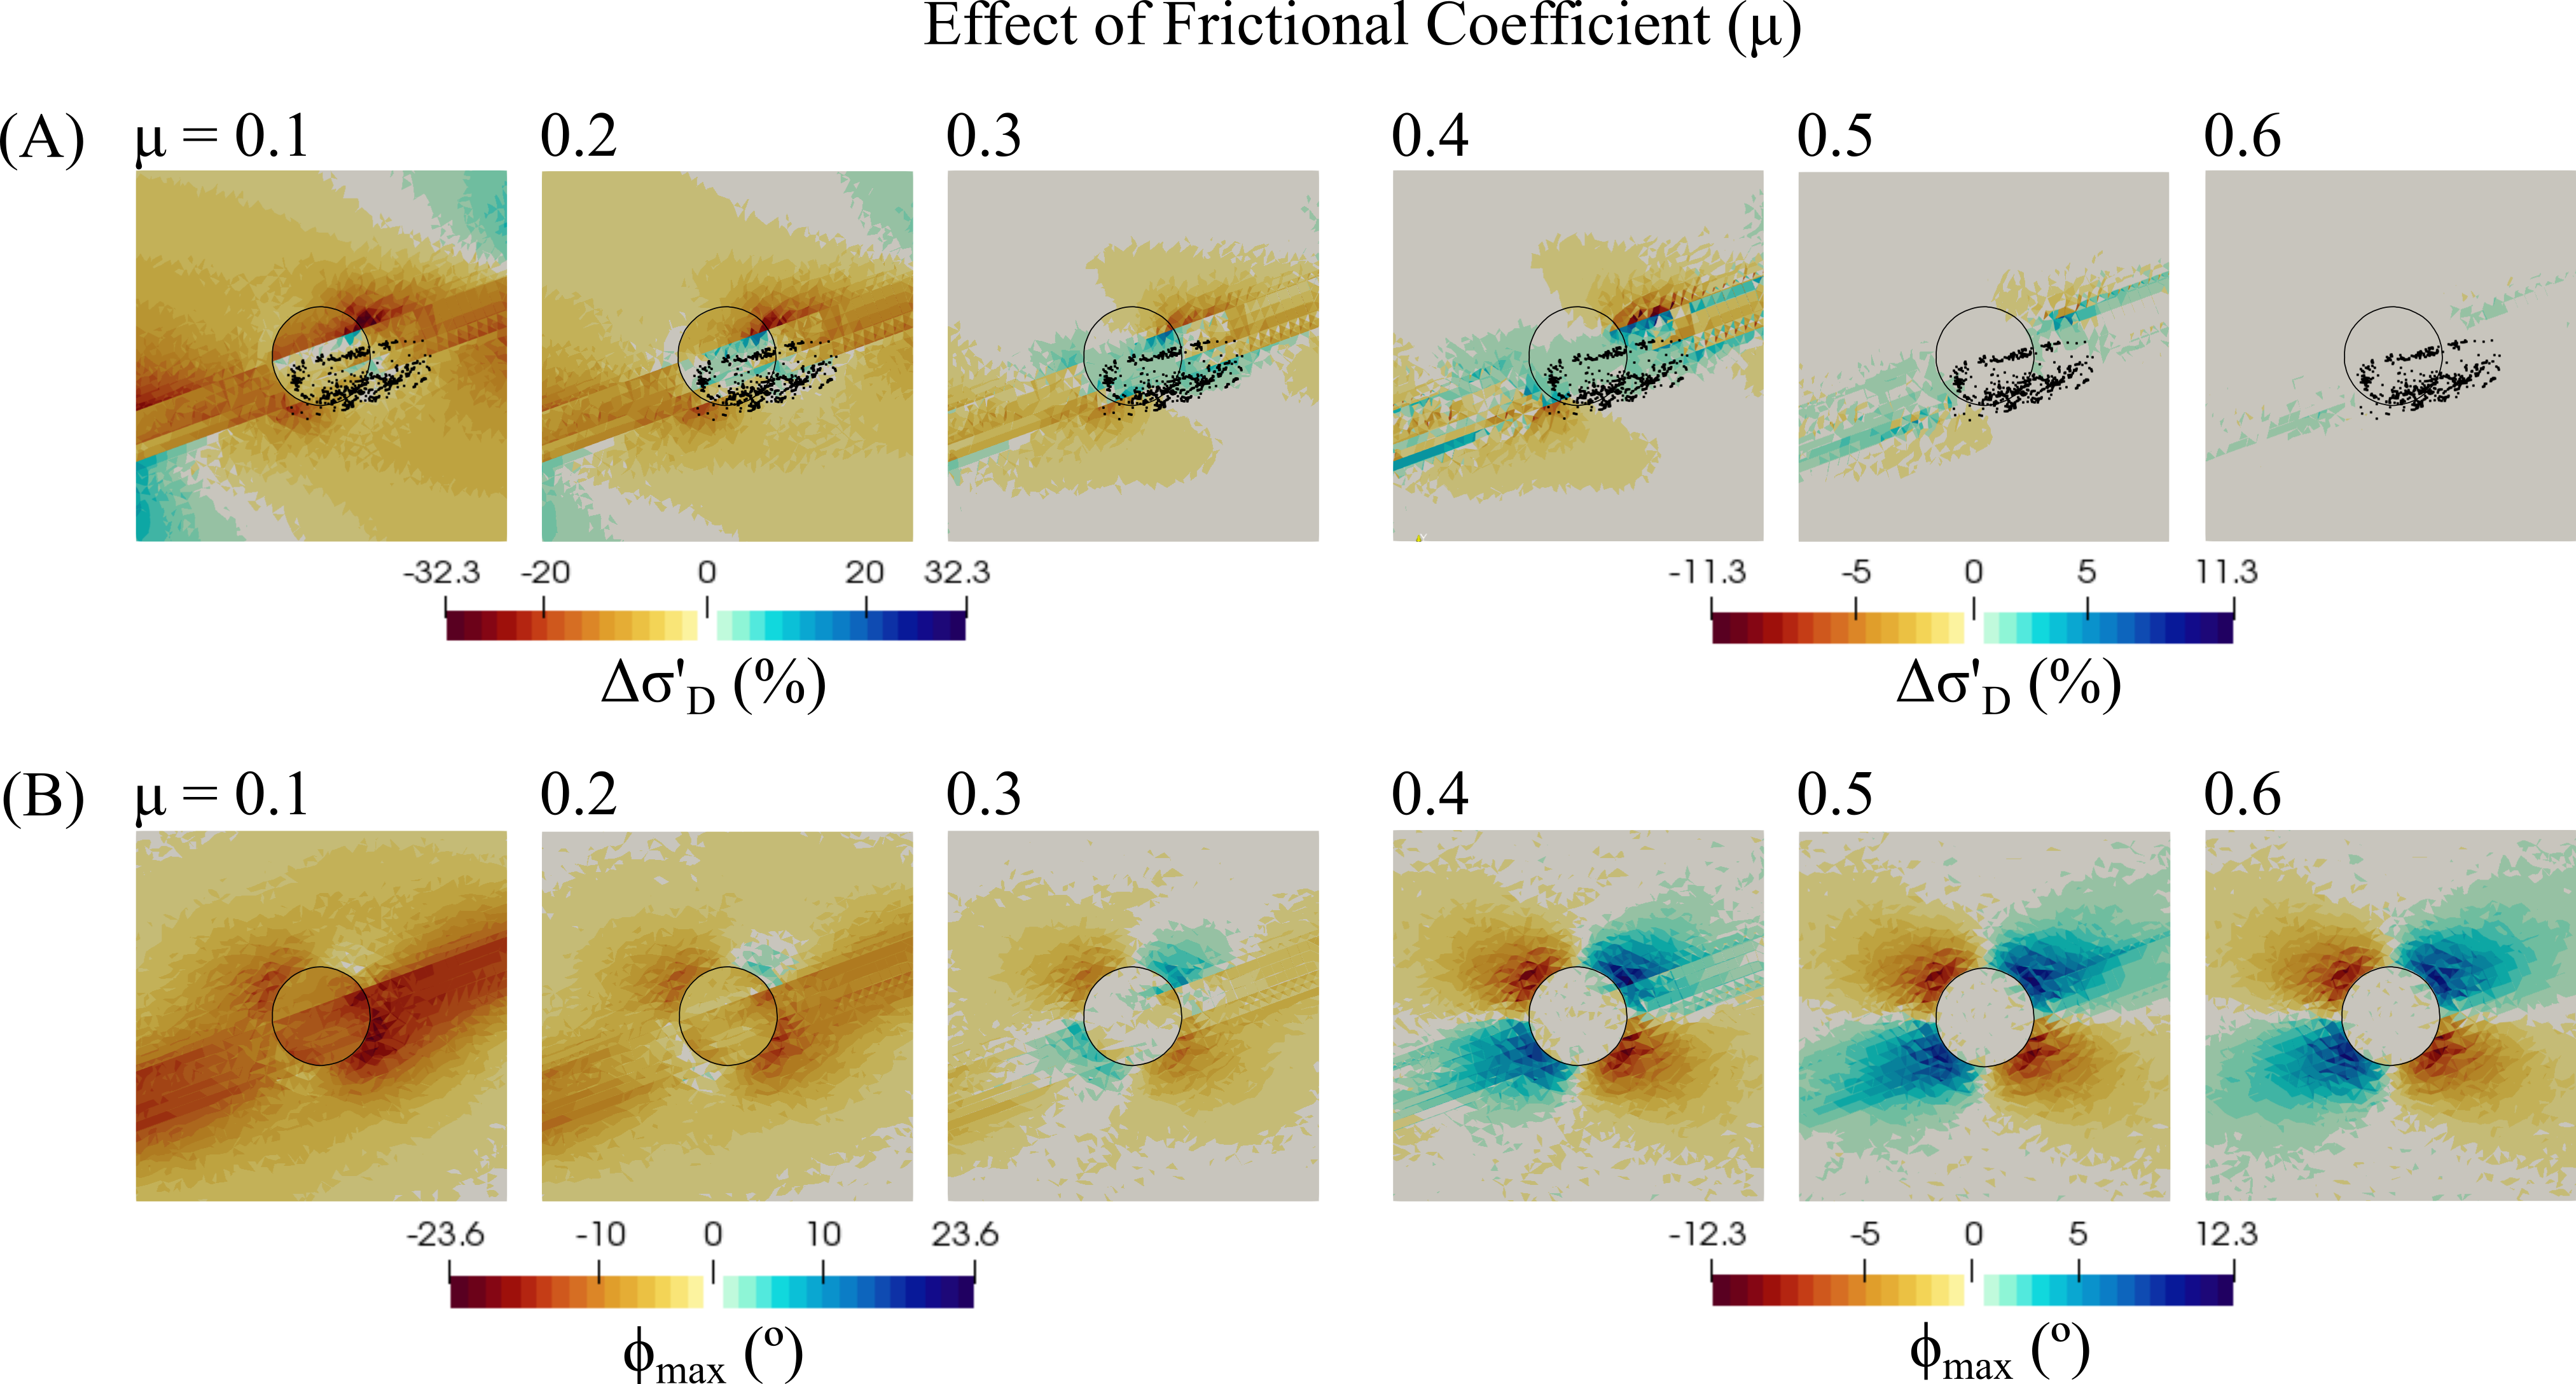
\includegraphics[width=30pc]{SD70R25V_2.png}
\caption{Effect of friction coefficient on the $\Delta\sigma_{D}^{\prime}$ and $\phi_{\max}$ in the SD70R25V model at 10 km depth. Note the change in scale for $\mu$ greater than 0.3. Earthquakes within 2 km of each depth slice are represented by black dots in \ref{fig:eff_of_mu}A. \add[OF]{The outline of the impact structure is represented as a black circle.} Each figure is 70 $\times$ 70 km.} 
\label{fig:eff_of_mu}
\end{figure}

$\phi_{\max}$ maps show a clockwise stress rotation in the entire seismic zone, including the \change[OF]{crater}{impact structure} region, when $\mu$ values are 0.1 and 0.2 (Fig. \ref{fig:eff_of_mu}B). When $\mu$ is 0.3, $\phi_{\max}$ is subparallel to the regional stress orientation within the \change[OF]{crater}{impact structure} region and the four-lobe pattern appears. For $\mu \ge$ 0.4, the distribution of $\phi_{\max}$ approaches that of the reference model.

% #########################################################################################################

\subsection{Effects of velocity models}
LD70R25 and TD70 are the same as SD70R25 except that they use different velocity models. We use the 1D velocity model \citep{lamontagne1999} (Fig.~\ref{figthree}) and the 3D tomography results \citep{Powell_2017} (Fig.~\ref{figfour}) in LD70R25 and TD70 models, respectively. The $V_p$ and $V_s$ tomography model covers and extends beyond the \change[OF]{crater}{impact structure} region, so the \change[OF]{crater}{impact structure}-crust elastic moduli ratio is irrelevant because it is dictated by the velocities.

\subsubsection{LD70R25}
Despite the difference in the 1D velocity models of \citet{lamontagne1999} and \citet{Somerville1990} especially at depths shallower than 20 km (Fig. \ref{figthree}), the results of LD70R25 are similar in spatial distribution and in magnitude to those of SD70R25 (Fig. \ref{fig:eff_of_vel}A). Regions of positive $\Delta\sigma_{D}^{\prime}$ spatially overlap with the observed seismicity at all depths and especially well at 10 km depth (Fig. \ref{fig:eff_of_vel}A).  

\begin{figure}[ht]
\centering
%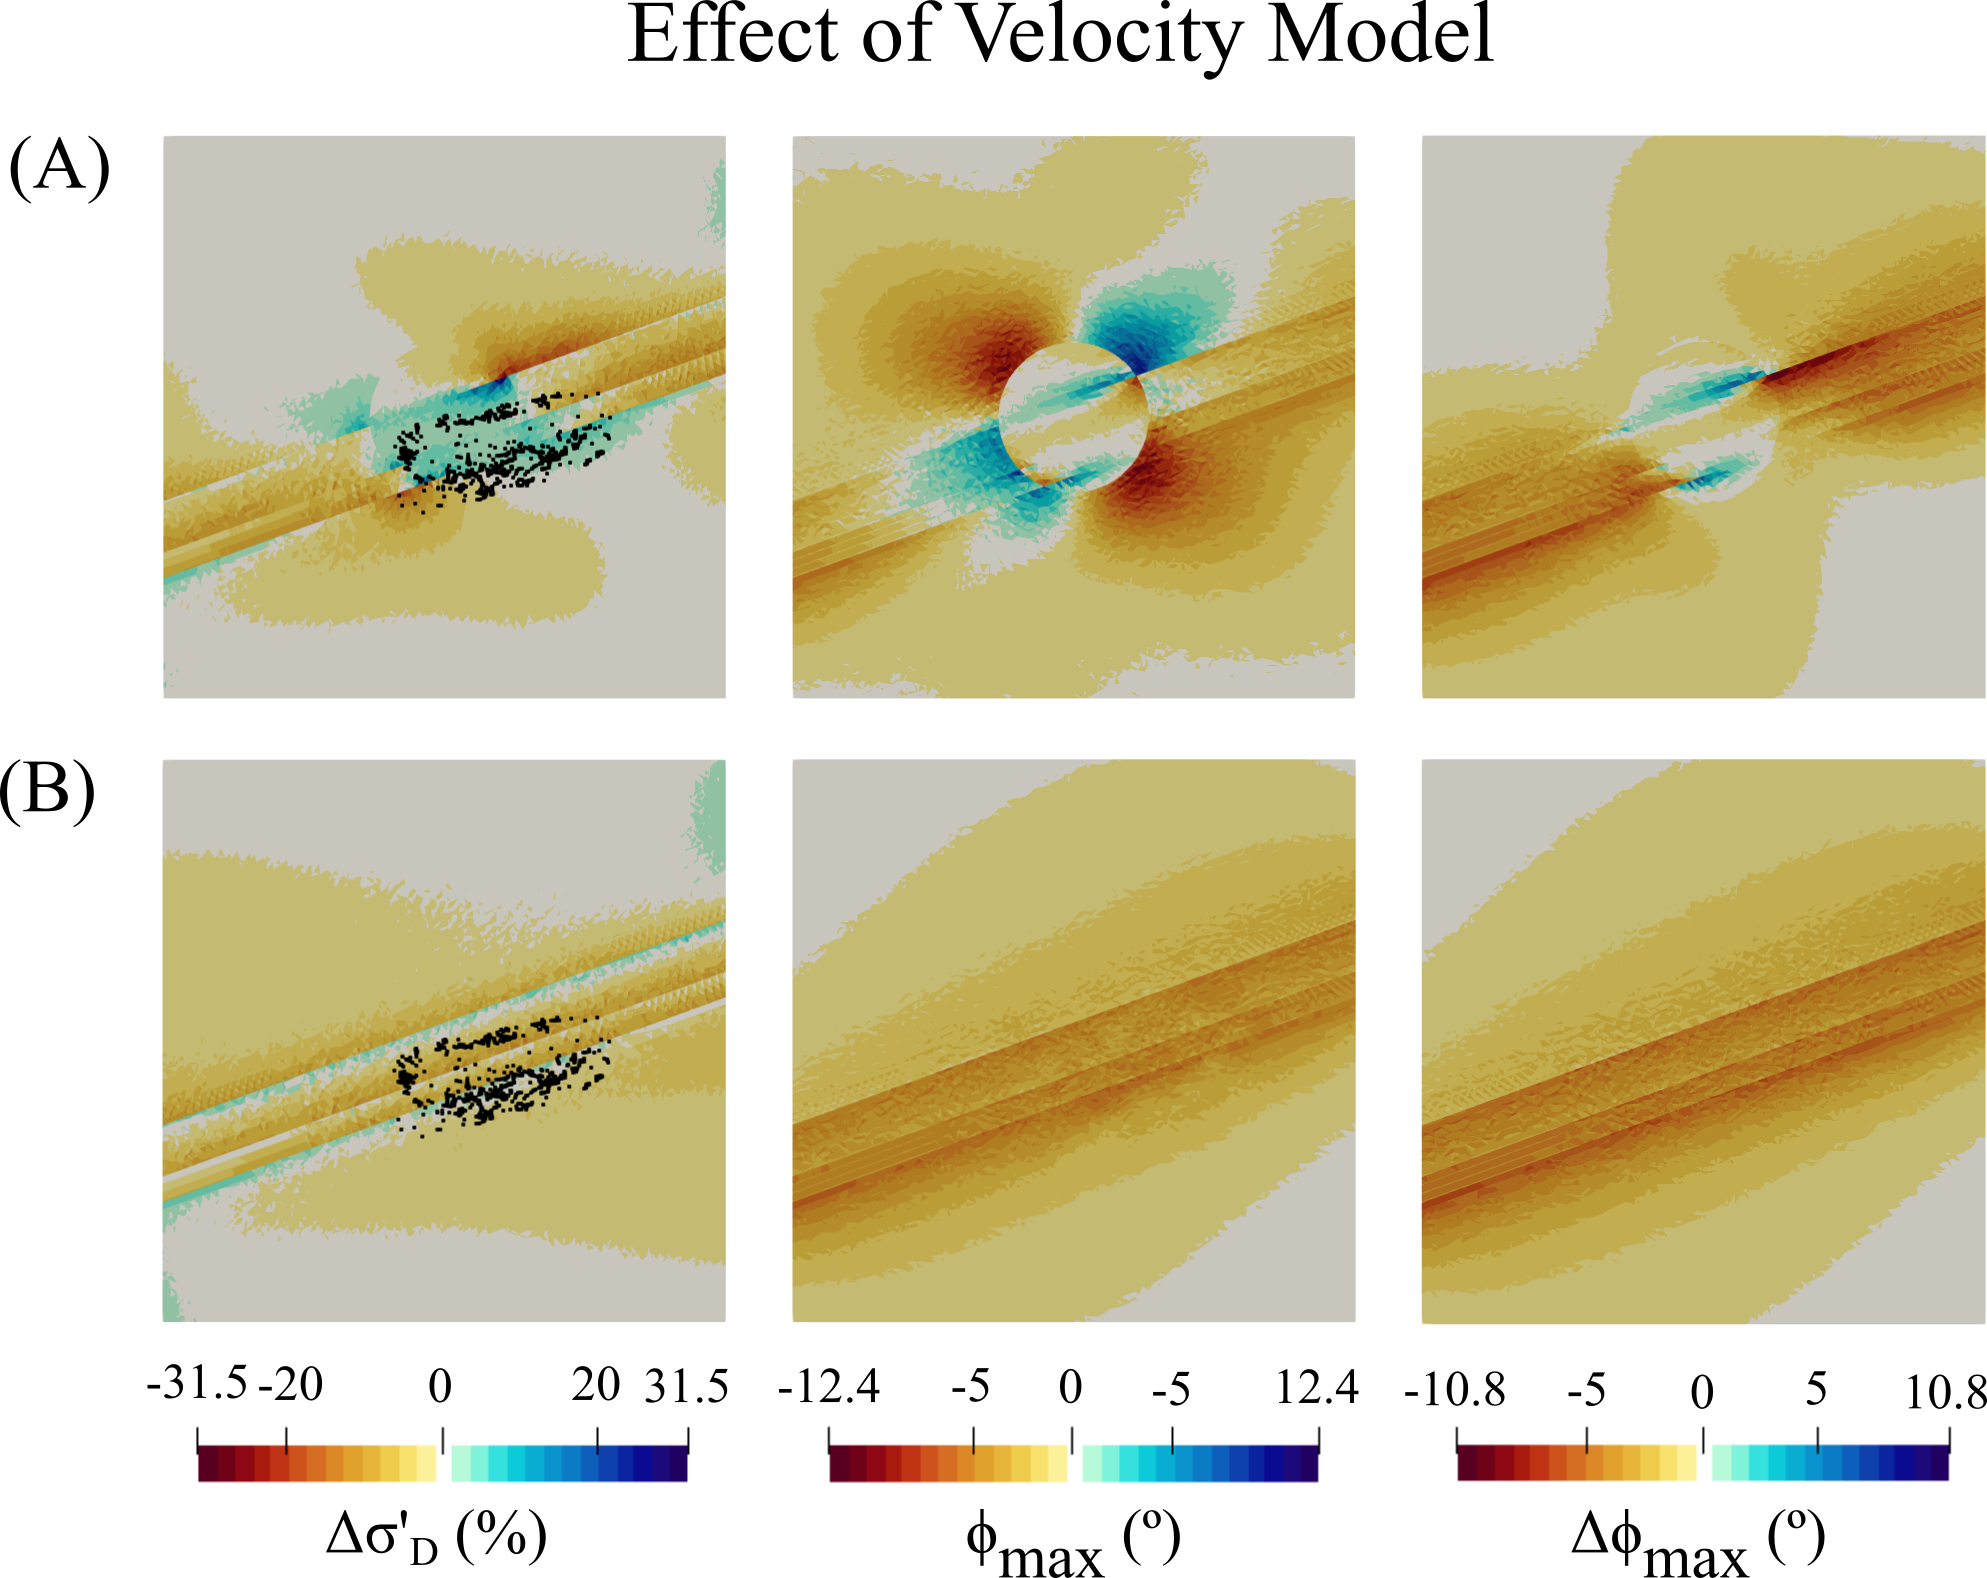
\includegraphics[width=20pc]{Figures/LD70R25_TD70.png}
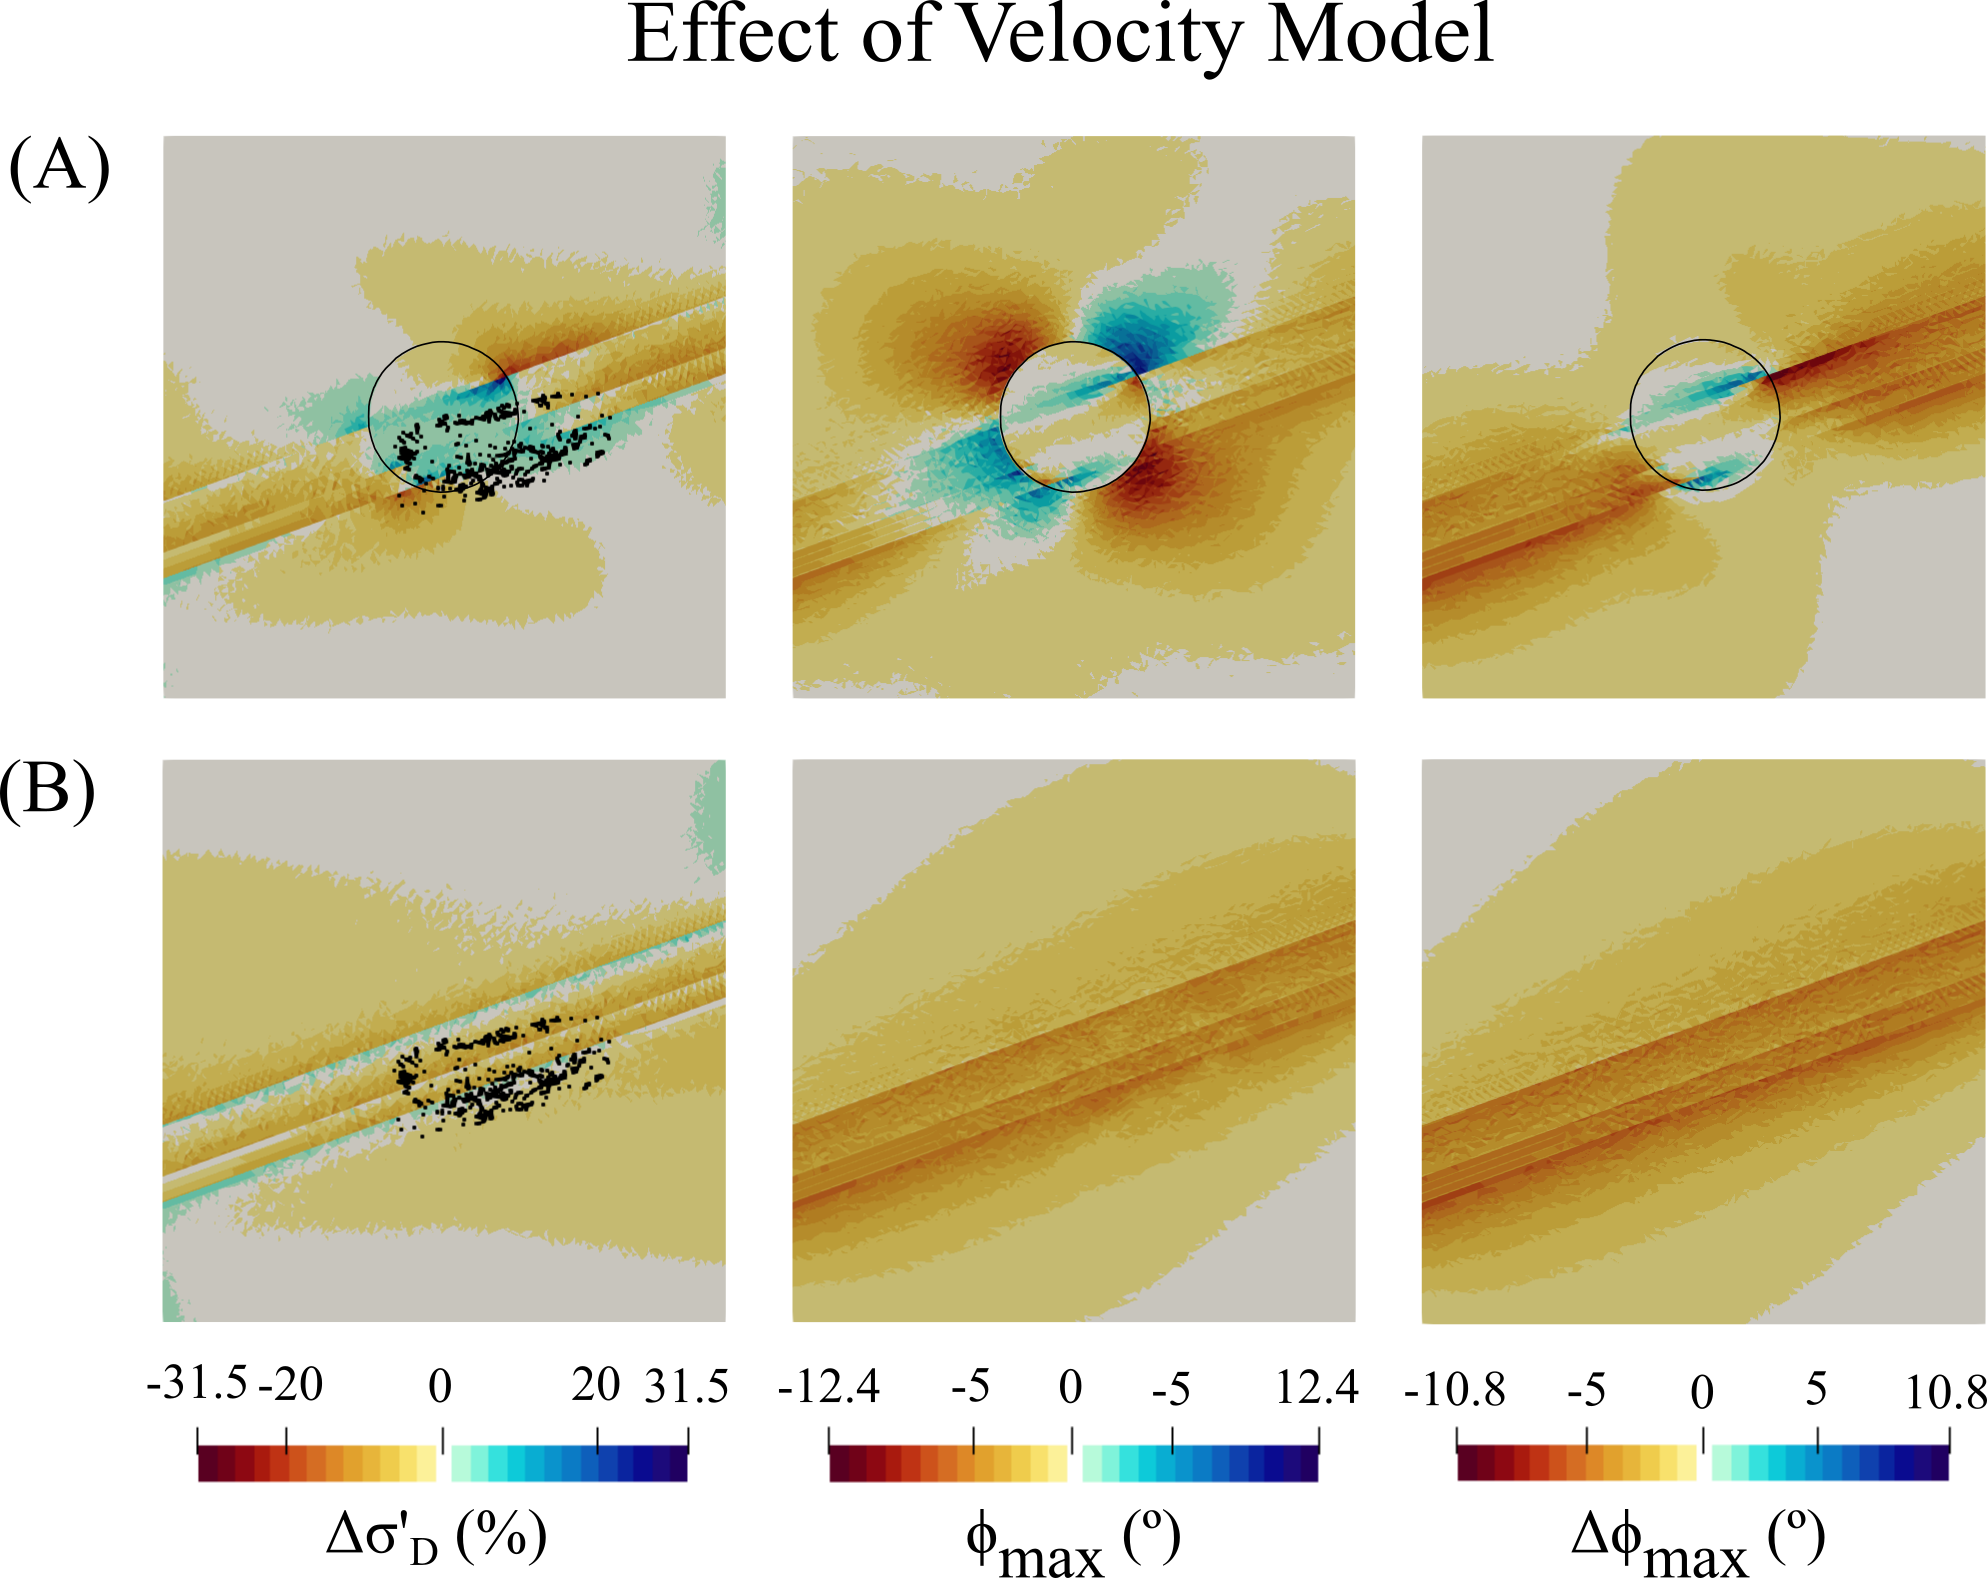
\includegraphics[width=20pc]{LD70R25_TD70_2.png}
\caption{Same as Fig.~\ref{fig:eff_of_dips} but only at a depth of 10 km for (A) LD70R25 and (B) TD70.}
\label{fig:eff_of_vel}
\end{figure}

The $\phi_{\max}$ maps also show the four-lobe pattern around the weaker \change[OF]{crater}{impact structure} and modification of the $\phi_{\max}$ by the rift faults is observed (Fig. \ref{fig:eff_of_vel}A). The maximum value of $\phi_{\max}$ is 21.7$^\circ$ and decreases to 12.4$^\circ$ at 10 km depth. The $\Delta\phi_{\max}$ map shows that the rotation of the reference model $\phi_{\max}$ due to the rift faults is up to 10.8$^\circ$ at 10 km depth (Fig. \ref{fig:eff_of_vel}A).


% #############################################################
\subsubsection{TD70}
TD70 shows very different results from those of the models with a layered velocity model and a weak \change[OF]{crater}{impact structure}. As the tomography model does not clearly show low velocities within the \change[OF]{crater}{impact structure} region, $\Delta\sigma_{D}^{\prime}$, $\phi_{\max}$ and $\Delta\phi_{\max}$ are all very similar to those in SD70R100, in which the \change[OF]{crater}{impact structure} is not distinguished from the surrounding crust in terms of elastic stiffness.

The spatial correlation between $\Delta\sigma_{D}^{\prime}$ and the observed seismicity is poor, especially at 10 km depths (Fig. \ref{fig:eff_of_vel}B). Below 15 km depths, the earthquakes fall within a region of positive $\Delta\sigma_{D}^{\prime}$ but the modeled distribution of $\Delta\sigma_{D}^{\prime}$ predicts earthquakes throughout the entire length of the rift faults. 


The $\phi_{\max}$ maps do not show the characteristic four-lobe pattern as seen in the models with the \change[OF]{crater}{impact structure} due to the lack of a significant decrease in the velocity model within the \change[OF]{crater}{impact structure} versus outside the \change[OF]{crater}{impact structure} (Fig. \ref{fig:eff_of_vel}B). The $\phi_{\max}$ maps show a clockwise rotation relative to the regional stress orientation up to 12.4$^\circ$ at 10 km depth (Fig. \ref{fig:eff_of_vel}B).

The $\Delta\phi_{\max}$ is similar in magnitude and in spatial distribution with the $\phi_{\max}$ maps (Fig. \ref{fig:eff_of_vel}B). This similarity in magnitude shows that the stress rotations in TD70 model are due to the presence of the rift faults.

% #############################################################
\section{Discussions}

\subsection{Earthquake distribution}
Our models suggest that having both the rift faults and the impact \change[OF]{crater}{structure} is not only sufficient but also necessary for explaining the distribution of earthquakes in the CSZ. The models without a weaker \change[OF]{crater}{impact structure} zone, SD70R100 and TD70, show regions of positive $\Delta \sigma_{D}^{\prime}$, a proxy for earthquake generation potential, along the entire length of the rift faults (e.g., Fig. \ref{fig:eff_of_moduli_ratio}B). In contrast, when the \change[OF]{crater}{impact structure} is set to be \change[OF]{less elastically stiff}{elastically softer} than the surrounding crust \add[OF]{ by up to a factor of 4}, positive $\Delta \sigma_{D}^{\prime}$ regions spatially coincide with the observed seismicity in the CSZ, especially above 15 km depth (e.g., Fig. \ref{fig:SD70R25}C). Our models predict that earthquake activity should extend to about 20 km \add[OF]{distance} from the \change[OF]{crater}{impact structure} in a northeast direction (Fig. \ref{fig:SD70R25}C). This distribution of positive $\Delta \sigma_{D}^{\prime}$ is not seen in the reference model without the rift faults. These two findings from our models are consistent with the conclusion drawn by~\citet{Thomas_Powell_2017} that the seismicity in CSZ requires both the damaged \change[OF]{crater}{impact structure} zone and the rift faults.

The SD70R25 and SD65R25 models can explain the seismicity of the CSZ at least partially (Figs.~\ref{fig:profiles_70_70_70_2km} and~\ref{fig:profiles_65_40_40_2km}). Correlation between the $\Delta\sigma_{D}^{\prime}$ distribution in SD65R25 and the observed seismicity shows a better and fine-scale correlation than in SD70R25, especially well near and within the \change[OF]{crater}{impact structure} region (Fig. \ref{fig:profiles_65_40_40_2km}) while those in SD70R25 fit the observed seismicity better in the northeast region outside the \change[OF]{crater}{impact structure} (Fig. \ref{fig:profiles_70_70_70_2km}). These differential correlations with seismicity of positive $\Delta \sigma_{D}^{\prime}$ regions in SD70R25 and SD65R25 might be suggesting along-strike variations in the dip angles of the rift faults~\citep[e.g.,][]{Baird_2010}. The SD65R25 model explains the observed seismic gap between the NW and SE clusters (i.e., between Gouffre Northwest and the Saint-Laurent faults, Fig. \ref{figone}) and can also explain the rimming of earthquakes around the \change[OF]{crater}{impact structure} as noted by~\citet{Powell_2017} especially at 10 km depth (Fig.~\ref{fig:profiles_65_40_40_2km}). 

Our present models, however, cannot explain the differences in earthquake activity between the \change[OF]{crater}{impact structure} and the surrounding crust in the CSZ. `b' values of the Gutenberg-Richter relationship for the regions within and outside the \change[OF]{crater}{impact structure} are 0.93 and 0.74, respectively~\citep{Yu_2016}, indicating a higher frequency of small magnitude earthquakes within the \change[OF]{crater}{impact structure}. Also, \change[OF]{the large-magnitude}{most M4+} earthquakes in the CSZ \change[OF]{occurred}{appear to occur} in the northeast region outside the \change[OF]{crater}{impact structure}~\citep[e.g.,][]{lamontagne1999,Powell_2017,Baird_2010}. \add[OF]{Reexamination of historical earthquakes in the Charlevoix area by}~\citet{Stevens1980} \add[OF]{shows that some M4+ earthquakes in the period 1924-1978 also occurred at the SE end of the impact structure.} Our models do not show significantly higher values of $\Delta\sigma_{D}^\prime$ in the seismogenic zone outside the \change[OF]{crater}{impact structure} relative to the regions within the impact \change[OF]{crater}{structure} (Fig. \ref{fig:SD70R25}C). A possible explanation is that faults created in the highly fractured \change[OF]{crater}{impact structure} region~\citep{RONDOT_2000} might have lower friction coefficients than the faults outside the \change[OF]{crater}{impact structure}. Stress build-up on those weaker \change[OF]{crater}{impact structure} faults can be quicker and smaller in magnitude than on faults outside the \change[OF]{crater}{impact structure} under the same tectonic loading, resulting in more numerous, smaller magnitude earthquakes within versus outside the \change[OF]{crater}{impact structure}.

\subsection{Spatial variations of SH$_{\max}$ orientation}
Stress orientations in the CSZ from focal mechanism stress inversions \citep{Zoback_1992,Mazzotti_2010} show relative clockwise rotations within the CSZ and in the CSZ relative to the regional stress orientation. A clockwise rotation of about 47$^\circ$ is observed in the SE relative to NW clusters of earthquakes and about 32$^\circ$ from the stress inversion of the entire CSZ earthquakes relative to the SH$_{\max}$ determined from borehole breakouts~\citep{Zoback_1992,Mazzotti_2010} (Fig. \ref{figone}).

Most of the earthquakes in the NW cluster are within the \change[OF]{crater}{impact structure} region and occur at about 10 km depth (Fig. \ref{figone}). Our model shows that the rift faults tend to rotate the stress orientation clockwise in the upper 15 km depth but the amount of rotation is reduced within the weak \change[OF]{crater}{impact structure} (e.g., Fig. \ref{fig:SD70R25}D). However, the model with a \change[OF]{crater}{impact structure}-crust moduli ratio of 1.0 shows significant clockwise rotations uniformly along the entire length of the rift faults (Fig. \ref{fig:eff_of_moduli_ratio}B). This observation suggests that the impact \change[OF]{crater}{structure} tends to align the $\phi_{\max}$ to the regional tectonic loading direction within the \change[OF]{crater}{impact structure}, particularly at 10 km depth (Fig. \ref{fig:SD70R25}D).

In a model with a \change[OF]{crater}{impact structure} and the rift faults (SD70R25), the stress rotation in the CSZ is clockwise (maximum value of 20.3$^\circ$) and decreases to 0$^\circ$ at an average of 20 km away from the CSZ (Fig. \ref{fig:SD70R25}B). SD70R25 can explain about 60$\%$ of the 32$^\circ$ clockwise stress rotation observed in the CSZ relative to the borehole breakouts, and about 43$\%$ of the 47$^\circ$ rotation in the SE part of the CSZ relative to the NW part. The magnitudes of $\phi_{\max}$ in the SD65R25 model are higher than the SD70R25 model by 6$^\circ$, but show a small clockwise rotation within the \change[OF]{crater}{impact structure} at 10 km depth, and thus can explain about 80$\%$ of the 32$^\circ$ clockwise stress rotation observed in the CSZ relative to the borehole breakouts, and about 55$\%$ of the 47$^\circ$ rotation in the SE part of the CSZ relative to the NW part. The increase in $\phi_{\max}$ in the SD65R25 relative to the SD70R25 models suggests that the remaining observed stress rotations, not explained by \change[OF]{both models}{either model}, could be partly due to change in dip angle of the rift faults with depth. 

A clockwise stress rotation of about 44$^\circ$ relative to the stress orientation from borehole breakouts is also observed in the Lower St Lawrence seismic zone \citep{Mazzotti_2010}. The Lower St. Lawrence seismic zone is located along the St. Lawrence River to the NE of the CSZ, and does not contain an impact \change[OF]{crater}{structure}, similar to the SD70R100 model. The rotation suggests that the presence of the rift faults and the relative angles of their strikes with respect to the regional orientation of SH$_{\max}$ alone can result in stress rotations ~\citep[e.g.,][]{Zoback_1992}. However, the combined effect of the impact \change[OF]{crater}{structure} with up to a quarter of the elastic moduli of the surrounding crust, and the rift faults are required in the CSZ to explain the observed clockwise rotations of the $\phi_{\max}$ in the SE cluster of earthquakes relative to the NW cluster, as well as in the entire CSZ relative to the direction of regional tectonic loading.


\subsection{Frictional strengths of the rift faults}
The surface expression of the rift faults used in this study correspond to the Gouffre Northwest Fault, Saint-Laurent fault and Charlevoix Fault (Fig. 1). We did not consider the South Shore fault given its aseismic nature \change[OF]{and its location at the extreme eastern edge of the crater}{, although it appears to mark a boundary to the active zone}~\citep{lamontagne1999}. Our models show that a $\mu$ of 0.3 and cohesion values of 0 MPa create $\Delta\sigma_{D}^\prime$ maps that spatially correlate with the seismicity of CSZ and the observed stress rotations (Fig. \ref{fig:eff_of_mu}). \add[OF]{We ran a series of models in which the rift faults dip at 70$^{\circ}$ and the friction coefficient ($\mu$) is fixed to be 0.3 while cohesion ($C$) is one of 0, 3, 5, 10, 20 and 30 MPa (Fig. S6). Cohesion values less than 5 MPa could better explain the spatial distribution of observed seismicity in the CSZ than the greater values.} \add[OF]{$\mu$ equal to 0.4 also seems suitable to the rift faults as the $\Delta\sigma_{D}^\prime$ maps spatially correlate well with the seismicity of the CSZ. A small number of earthquakes also occurred at the SW region outside the impact structure (Fig. $\ref{figone}$)}.
%, however, previous studies in the CSZ agreed with a finite extent of the seismicity}~\citep[e.g.,][]{Stevens1980}. \note[EC]{I don't understand the point of the sentence about the finite extent of the seismicity. Is it necessary?}\change[OF]{This}{Our fault model} is different from the work of \citet{Baird_2010} who modeled the Gouffre Northwest Fault, Saint-Laurent fault and South Shore Fault (Fig. \ref{figone}). \note[EC]{This sentence should be in the model setup unless you want to discuss implications of this difference.}

The fault parameters in our study are not compatible with the analysis of \citet{Hurd_Zoback_2012,Hurd_Zoback2012b} who suggest normal values of $\mu$ (0.6 $-$ 0.8) for the rift faults and hydrostatic pore pressure. Also, \citet{Fereidoni2014} use Coulomb stress theory to investigate stress change in the CSZ caused by the 1663 earthquake (moment magnitude M of 7) and conclude that the rift faults are strong with $\mu$ of 0.8. \citet{Fereidoni2014} showed that decreasing the apparent coefficient of friction reduces the spatial correlation of the regions with enhanced stress and observed seismicity. Specifically, $\mu$ values of 0.2 and 0.4 give 66$\%$ and 75$\%$ spatial correlation, respectively. However, in our model, the regions of positive $\Delta\sigma_{D}^\prime$ significantly decrease in spatial extent when $\mu$ is 0.6, and do not fit the observed seismicity in the CSZ (Fig. \ref{fig:eff_of_mu}).

\remove[OF]{In contrast to the normal faults as suggested by} 
%\citet{Hurd_Zoback_2012,Hurd_Zoback2012b,Fereidoni2014}, \citet{Baird_2010} 
\remove[OF]{conclude that the rift faults in the CSZ are very weak with a friction angle of 5$^\circ$ that is equivalent to a $\mu$ of about 0.1. This very low value of $\mu$ was necessary for their stopping criterion for boundary loading, which was $\sigma_{D}$ equal to 200 MPa at 10 km depth.} In our study, we stop increasing boundary displacements when $\sigma_{D}$ reaches 706 MPa at 10 km depth as described earlier without making any assumptions for the intermediate principal stress ($\sigma_2$). \add[OF]{In contrast,} \citet{Baird_2010} \add[OF]{used a $\sigma_{D}$ equal to 200 MPa at 10 km depth as their stopping criterion for boundary loading. They suggested that the rift faults in the CSZ are very weak with %a friction angle of 5$^\circ$ that is equivalent to 
a $\mu$ of about 0.1. The higher stopping criterion in our study is based on Byerlee's law under the assumption of no pore-fluid pressure on the rift faults, and it is necessary to make faults slip at seismogenic depth when $\mu$ is 0.3 as assumed in this study. Inclusion of pore-fluid pressure can significantly reduce the magnitude of $\sigma_{D}$ used as the stopping criterion. In other words, the lower stopping criterion, $\sigma_{D}$ equal to 200 MPa at 10 km depth, might be sufficient for rifts faults with $\mu$ = 0.3 or 0.4 to slip if pore fluid pressure is sufficiently high. Another possible consequences of pore-fluid pressure is that faults could be reactivated at smaller angles from the maximum compressive stress}~\citep[e.g.,][]{ChenChen18}.

%This very low value of $\mu$ was necessary for faults to slip under the stopping criterion for boundary loading, which was $\sigma_{D}$ equal to 200 MPa at 10 km depth. \add[OF]{
%, which will act to reduce the effective normal stress on the rift faults 
%Pore-fluid pressure is related to the lithostatic stress ($\rho g z$) by a pore-fluid factor ($\lambda$)~\citep[e.g.,][]{HubbertRubey1959, ZobackTownend2001}. $\lambda$ values are different for different pore-pressure states: e.g., for a hydrostatic state where pore spaces are interconnected up to the water table, $\labmda$ is between 0.3 and 0.4; for a suprahydrostatic state, $0.4 < \lambda \le 1.0$; and for the lithostatic state, $\lambda = 1.0$~\citep[e.g.,][]{Sibson2000,SibsonRowland,PetriniPodladchikov}. It has been suggested that seismic faulting in intraplate seismic zones generally occurs under hydrostatic fluid pressure conditions~$\citep{TownendZoback2000,SibsonRowland}$, except in areas of strong fluid release where $\lambda$ can be up to 1.0~$\citep{ManningIngebritsen99}$.% by up to a factor of two the value of the pore-fluid pressure~\citep[e.g.,][]{ZobackTownend2001}


\subsection{Velocity model of the CSZ}
Our models show that a 1D velocity model of the CSZ \citep{lamontagne1999} (Fig. \ref{figthree}) with embedded \change[OF]{crater}{impact structure} and rift faults can explain the observed seismicity and more than 50$\%$ of the stress rotations (Fig. \ref{fig:eff_of_vel}A). Using the velocity model of the \change[OF]{Sanguenay}{Saguenay} region does not improve this result (Fig. \ref{fig:SD70R25}). Similarly, $\Delta\sigma_{D}^\prime$ in the TD70 model did not spatially fit the recorded earthquakes in the upper 10 km in the CSZ because the distinct and lower-strength damaged zone is not apparent in the 3D tomography \citep{Powell_2017} (Fig. \ref{fig:eff_of_vel}B). \citet{lamontagne1999} \change[OF]{Further investigation is needed to determine why the supposedly better velocity models fail}{constructed a 1-D velocity model for the Canadian Shield region that does not include lateral variations of} velocity model to explain the seismicity and stress orientations.

\subsection{Limitations of our study}
Our models could not explain some earthquakes in the SW part of the \change[OF]{crater}{impact structure} especially in the upper 10 km depth (Fig. \ref{fig:SD70R25}C). We did not account for stress changes due to a large historic earthquake in the CSZ and the postglacial rebound as modeled by \citet{Fereidoni2014} and \citet{Mazzotti_GPS2005}, respectively.

Our models can only explain about 50\% of the observed $SH_{\max}$ rotation. A possible hypothesis for the remaining stress rotation is a change in the dip of the rift faults with depth and the effect of postglacial rebound. \remove[OF]{The high stress rotation could also be due to unconstrained focal mechanisms used in the stress inversion.} Most of the focal mechanisms used for stress inversion \add[OF]{in the CSZ} are obtained from first motion P and SH waves~\citep{Mazzotti_2010,lamontagne1998}. \change[OF]{Better constrained}{The} focal mechanisms %\note[EC]{What do you mean by ``focal mechanisms are `good\rq{}''? It would be good/nice to have better constrained ones, you mean?}
\add[OF]{are well defined, and we suggest that the focal mechanisms can be further constrained} using waveform modeling \remove[OF]{will be needed} to validate the magnitude of the stress rotation.

We \change[OF]{simplified}{assumed that} the rift faults to be planar however, the fault \change[OF]{trace}{traces} on the geologic map of the CSZ \change[OF]{is not straight}{are not linear} (Fig. \ref{figone}). The scatter of the seismicity within the \change[OF]{crater}{impact structure} indicates that the faults do not remain planar. Future models depicting a more realistic fault geometry may also shed light on the factors controlling stress rotation. Our model also did not incorporate pore pressure which could have affected the calculated $\mu$ \add[OF]{and maximum $\sigma_{D}$}.
The 3D velocity model is not \change[OF]{accurate}{very well defined} in the upper 5 km depth and does not cover the entire seismic zone (Fig. \ref{figfour}).


% #############################################################
\section{Conclusions}
Findings from this study can be summarized as follows:

\begin{itemize}

\item The combined effects of the impact \change[OF]{crater}{impact structure} and the rift faults are required in the CSZ to explain the observed distribution of seismicity and more than 50$\%$ of the observed clockwise rotations of the $\phi_{\max}$ in the CSZ \add[OF]{with respect to the regional maximum compressive stress direction}.

\item \change[OF]{A crater}{An impact structure} elastically weaker than the surrounding crust by up to a factor of 4 is required to explain the seismicity in the upper 10 km of the CSZ and the observed clockwise rotation of the SH$_{\max}$ in the SE relative to the NW part of the \change[OF]{crater}{impact structure}. Below 10 km depth in the \change[OF]{crater}{impact structure}, reactivation of the rift faults explains the observed seismicity in the CSZ.

\item Stress models that spatially correlate with the seismicity of CSZ and the observed stress rotations were obtained when rifts faults have a friction coefficient of 0.3 and zero cohesion \add[OF]{under an assumption of no pore-fluid pressure on the rift faults}.

\item The magnitudes of SH$_{\max}$ rotation are greater in the 65$^\circ$-40$^\circ$-40$^\circ$ fault dip case than the constant 70$^\circ$ fault dip case by 6$^\circ$. The remaining SH$_{\max}$ rotation could be due to a change in the dip of the rift faults with depth.

\item Stress models with dips of 65$^\circ$, 40$^\circ$ and 40$^\circ$ based on a recent hypocenter relocation study show a better correlation between the high differential stress regions and the observed seismicity near and within the \change[OF]{crater}{impact structure} region than those with a constant 70$^\circ$ dip. However, the constant-dip models fit the observed seismicity better in the northeast region outside the \change[OF]{crater}{impact structure}. The partial success of each model might indicate more complex geometry of the faults: e.g., an along-strike variation of the dip angles of the rift faults.
 
\end{itemize}


%%%%%%%%%%%%%%
% Acronyms
\begin{acronyms}
 \acro{CSZ}
  Charlevoix Seismic Zone
 \acro{SH$_{\max}$}
  Maximum horizontal principal stress 
\end{acronyms}


%%%%%%%%%%%%%%
\acknowledgments
This project is supported by the National Science Foundation (NSF - ICER) under the award title ``EarthCube Building Blocks: Collaborative Proposal: GeoTrust: Improving Sharing and Reproducibility of Geoscience Applications'' with an award number 1639706. We acknowledge the high performance computing (HPC) resource center at the University of Memphis, TN for providing the computing time for this research. \add[OF]{Earthquake dataset are available from Earthquakes Canada, GSC, Earthquake Search (On-line Bulletin), http://earthquakescanada.nrcan.gc.ca/stndon/NEDB-BNDS/bulletin-en.php, Natural Resources Canada (1/30/2019).}

%%%%%%%%%%%%%%
% Citation
%% Example \citet and \citep:
%  ...as shown by \citet{Boug10}, \citet{Buiz07}, \citet{Fra10},
%  \citet{Ghel00}, and \citet{Leit74}. 

%  ...as shown by \citep{Boug10}, \citep{Buiz07}, \citep{Fra10},
%  \citep{Ghel00, Leit74}. 

%  ...has been shown \citep [e.g.,][]{Boug10,Buiz07,Fra10}.

\bibliography{biblio}

    
%%%%%%%%%%%%%%%%%%%%%%%%%%%%%%%%%%%%%%%%%%%%%%%


%%

%  Numbered lines in equations:
%  To add line numbers to lines in equations,
%  \begin{linenomath*}
%  \begin{equation}
%  \end{equation}
%  \end{linenomath*}

%% Enter Figures and Tables near as possible to where they are first mentioned:
%
% DO NOT USE \psfrag or \subfigure commands.
%
% Figure captions go below the figure.
% Table titles go above tables;  other caption information
%  should be placed in last line of the table, using
% \multicolumn2l{$^a$ This is a table note.}
%
%----------------
% EXAMPLE FIGURE
%
% \begin{figure}[h]
% \centering
% when using pdflatex, use pdf file:
% \includegraphics[width=20pc]{figsamp.pdf}
%
% when using dvips, use .eps file:
% \includegraphics[width=20pc]{figsamp.eps}
%
% \caption{Short caption}
% \label{figone}
%  \end{figure}
%
% ---------------
% EXAMPLE TABLE
%
% \begin{table}
% \caption{Time of the Transition Between Phase 1 and Phase 2$^{a}$}
% \centering
% \begin{tabular}{l c}
% \hline
%  Run  & Time (min)  \\
% \hline
%   $l1$  & 260   \\
%   $l2$  & 300   \\
%   $l3$  & 340   \\
%   $h1$  & 270   \\
%   $h2$  & 250   \\
%   $h3$  & 380   \\
%   $r1$  & 370   \\
%   $r2$  & 390   \\
% \hline
% \multicolumn{2}{l}{$^{a}$Footnote text here.}
% \end{tabular}
% \end{table}

%% SIDEWAYS FIGURE and TABLE 
% AGU prefers the use of {sidewaystable} over {landscapetable} as it causes fewer problems.
%
% \begin{sidewaysfigure}
% \includegraphics[width=20pc]{figsamp}
% \caption{caption here}
% \label{newfig}
% \end{sidewaysfigure}
% 
%  \begin{sidewaystable}
%  \caption{Caption here}
% \label{tab:signif_gap_clos}
%  \begin{tabular}{ccc}
% one&two&three\\
% four&five&six
%  \end{tabular}
%  \end{sidewaystable}

%% If using numbered lines, please surround equations with \begin{linenomath*}...\end{linenomath*}
%\begin{linenomath*}
%\begin{equation}
%y|{f} \sim g(m, \sigma),
%\end{equation}
%\end{linenomath*}

%%% End of body of article

%%%%%%%%%%%%%%%%%%%%%%%%%%%%%%%%
%% Optional Appendix goes here
%
% The \appendix command resets counters and redefines section heads
%
% After typing \appendix
%
%\section{Here Is Appendix Title}
% will show
% A: Here Is Appendix Title
%
%\appendix
%\section{Here is a sample appendix}

%%%%%%%%%%%%%%%%%%%%%%%%%%%%%%%%%%%%%%%%%%%%%%%%%%%%%%%%%%%%%%%%
%
% Optional Glossary, Notation or Acronym section goes here:
%
%%%%%%%%%%%%%%  
% Glossary is only allowed in Reviews of Geophysics
%  \begin{glossary}
%  \term{Term}
%   Term Definition here
%  \term{Term}
%   Term Definition here
%  \term{Term}
%   Term Definition here
%  \end{glossary}

%
%%%%%%%%%%%%%%
% Acronyms
%\begin{acronyms}
% \acro{CSZ}
%  Charlevoix Seismic Zone
% \acro{SH$_{max}$}
%  Maximum horinzontal principal stress 
%\end{acronyms}

%
%%%%%%%%%%%%%%
% Notation 
%   \begin{notation}
%   \notation{$a+b$} Notation Definition here
%   \notation{$e=mc^2$} 
%   Equation in German-born physicist Albert Einstein's theory of special
%  relativity that showed that the increased relativistic mass ($m$) of a
%  body comes from the energy of motion of the body—that is, its kinetic
%  energy ($E$)—divided by the speed of light squared ($c^2$).
%   \end{notation}




%%%%%%%%%%%%%%%%%%%%%%%%%%%%%%%%%%%%%%%%%%%%%%%%%%%%%%%%%%%%%%%%
%
%  ACKNOWLEDGMENTS
%
% The acknowledgments must list:
%
% •	All funding sources related to this work from all authors
%
% •	Any real or perceived financial conflicts of interests for any
%	author
%
% •	Other affiliations for any author that may be perceived as
% 	having a conflict of interest with respect to the results of this
% 	paper.
%
% •	A statement that indicates to the reader where the data
% 	supporting the conclusions can be obtained (for example, in the
% 	references, tables, supporting information, and other databases).
%
% It is also the appropriate place to thank colleagues and other contributors. 
% AGU does not normally allow dedications.








%% ------------------------------------------------------------------------ %%
%% Citations

% Please use ONLY \citet and \citep for reference citations.
% DO NOT use other cite commands (e.g., \cite, \citeyear, \nocite, \citealp, etc.).


%% Example \citet and \citep:
%  ...as shown by \citet{Boug10}, \citet{Buiz07}, \citet{Fra10},
%  \citet{Ghel00}, and \citet{Leit74}. 

%  ...as shown by \citep{Boug10}, \citep{Buiz07}, \citep{Fra10},
%  \citep{Ghel00, Leit74}. 

%  ...has been shown \citep [e.g.,][]{Boug10,Buiz07,Fra10}.



%%  REFERENCE LIST AND TEXT CITATIONS
%
% Either type in your references using
%
% \begin{thebibliography}{}
% \bibitem[{\textit{Kobayashi et~al.}}(2003)]{R2013} Kobayashi, T.,
% Tran, A.~H., Nishijo, H., Ono, T., and Matsumoto, G.  (2003).
% Contribution of hippocampal place cell activity to learning and
% formation of goal-directed navigation in rats. \textit{Neuroscience}
% 117, 1025--1035.
%
% \bibitem{}
% Text
% \end{thebibliography}
%
%%%%%%%%%%%%%%%%%%%%%%%%%%%%%%%%%%%%%%%%%%%%%%%
% Or, to use BibTeX:
%
% Follow these steps
%
% 1. Type in \bibliography{<name of your .bib file>} 
%    Run LaTeX on your LaTeX file.
%
% 2. Run BiBTeX on your LaTeX file.
%
% 3. Open the new .bbl file containing the reference list and
%   copy all the contents into your LaTeX file here.
%
% 4. Run LaTeX on your new file which will produce the citations.
%
% AGU does not want a .bib or a .bbl file. Please copy in the contents of your .bbl file here.

%\bibliography{bibliography/biblio} 

%% After you run BibTeX, Copy in the contents of the .bbl file here:

\end{document}

%%%%%%%%%%%%%%%%%%%%%%%%%%%%%%%%%%%%%
%% Supporting Information
%% (Optional) See AGUSuppInfoSamp.tex/pdf for requirements 
%% for Supporting Information.
%%%%%%%%%%%%%%%%%%%%%%%%%%%%%%%%%%%%%



%%%%%%%%%%%%%%%%%%%%%%%%%%%%%%%%%%%%%%%%%%%%%%%%%%%%%%%%%%%%%%%

More Information and Advice:

%% ------------------------------------------------------------------------ %%
%
%  SECTION HEADS
%
%% ------------------------------------------------------------------------ %%

% Capitalize the first letter of each word (except for
% prepositions, conjunctions, and articles that are
% three or fewer letters).

% AGU follows standard outline style; therefore, there cannot be a section 1 without
% a section 2, or a section 2.3.1 without a section 2.3.2.
% Please make sure your section numbers are balanced.
% ---------------
% Level 1 head
%
% Use the \section{} command to identify level 1 heads;
% type the appropriate head wording between the curly
% brackets, as shown below.
%
%An example:
%\section{Level 1 Head: Introduction}
%
% ---------------
% Level 2 head
%
% Use the \subsection{} command to identify level 2 heads.
%An example:
%\subsection{Level 2 Head}
%
% ---------------
% Level 3 head
%
% Use the \subsubsection{} command to identify level 3 heads
%An example:
%\subsubsection{Level 3 Head}
%
%---------------
% Level 4 head
%
% Use the \subsubsubsection{} command to identify level 3 heads
% An example:
%\subsubsubsection{Level 4 Head} An example.
%
%% ------------------------------------------------------------------------ %%
%
%  IN-TEXT LISTS
%
%% ------------------------------------------------------------------------ %%
%
% Do not use bulleted lists; enumerated lists are okay.
% \begin{enumerate}
% \item
% \item
% \item
% \end{enumerate}
%
%% ------------------------------------------------------------------------ %%
%
%  EQUATIONS
%
%% ------------------------------------------------------------------------ %%

% Single-line equations are centered.
% Equation arrays will appear left-aligned.

Math coded inside display math mode \[ ...\]
 will not be numbered, e.g.,:
 \[ x^2=y^2 + z^2\]

 Math coded inside \begin{equation} and \end{equation} will
 be automatically numbered, e.g.,:
 \begin{equation}
 x^2=y^2 + z^2
 \end{equation}


% To create multiline equations, use the
% \begin{eqnarray} and \end{eqnarray} environment
% as demonstrated below.
\begin{eqnarray}
  x_{1} & = & (x - x_{0}) \cos \Theta \nonumber \\
        && + (y - y_{0}) \sin \Theta  \nonumber \\
  y_{1} & = & -(x - x_{0}) \sin \Theta \nonumber \\
        && + (y - y_{0}) \cos \Theta.
\end{eqnarray}

%If you don't want an equation number, use the star form:
%\begin{eqnarray*}...\end{eqnarray*}

% Break each line at a sign of operation
% (+, -, etc.) if possible, with the sign of operation
% on the new line.

% Indent second and subsequent lines to align with
% the first character following the equal sign on the
% first line.

% Use an \hspace{} command to insert horizontal space
% into your equation if necessary. Place an appropriate
% unit of measure between the curly braces, e.g.
% \hspace{1in}; you may have to experiment to achieve
% the correct amount of space.


%% ------------------------------------------------------------------------ %%
%
%  EQUATION NUMBERING: COUNTER
%
%% ------------------------------------------------------------------------ %%

% You may change equation numbering by resetting
% the equation counter or by explicitly numbering
% an equation.

% To explicitly number an equation, type \eqnum{}
% (with the desired number between the brackets)
% after the \begin{equation} or \begin{eqnarray}
% command.  The \eqnum{} command will affect only
% the equation it appears with; LaTeX will number
% any equations appearing later in the manuscript
% according to the equation counter.
%

% If you have a multiline equation that needs only
% one equation number, use a \nonumber command in
% front of the double backslashes (\\) as shown in
% the multiline equation above.

% If you are using line numbers, remember to surround
% equations with \begin{linenomath*}...\end{linenomath*}

%  To add line numbers to lines in equations:
%  \begin{linenomath*}
%  \begin{equation}
%  \end{equation}
%  \end{linenomath*}
